%File: formatting-instruction.tex
\documentclass[letterpaper]{article}
\usepackage{aaai}
\usepackage{times}
\usepackage{helvet}
\usepackage{courier}
\usepackage{amsmath}
\usepackage{amsfonts}
\usepackage{graphicx}
\usepackage{xcolor}
\usepackage{float}
\usepackage{siunitx}
\usepackage{multirow}
\usepackage{hyperref}
\newtheorem{hyp}{Hypothesis}
\DeclareMathOperator*{\argmax}{arg\,max}
\DeclareMathOperator*{\argmin}{arg\,min}

\frenchspacing
\setlength{\pdfpagewidth}{8.5in}
\setlength{\pdfpageheight}{11in}
\pdfinfo{
/Title (Insert Your Title Here)
/Author (Put All Your Authors Here, Separated by Commas)}
\setcounter{secnumdepth}{0}  
 \begin{document}
% The file aaai.sty is the style file for AAAI Press 
% proceedings, working notes, and technical reports.
%
\title{That and There: Judging the Intent of Pointing Actions with Robotic Arms}

% \title{Interpretation of Pointing Action: Expressing the intent of pick-and-place task}

% \author{AAAI Press\\
% Association for the Advancement of Artificial Intelligence\\
% 2275 East Bayshore Road, Suite 160\\
% Palo Alto, California 94303\\
% }

\author{Malihe Alikhani \quad  Baber Khalid* \quad Rahul Shome* \quad Chaitanya Mitash \quad Kostas Bekris \quad Matthew Stone\\
  Computer Science, \quad Rutgers University, \quad {\tt\small firstname.lastname@rutgers.edu}}
  
\maketitle
\begin{abstract}
\begin{quote}

Collaborative robotics requires effective communication between a robot and a human partner. This work proposes a set of interpretive principles for how a robotic arm can use pointing actions to communicate task information to people by extending existing models from the related literature. These principles are evaluated through studies where English-speaking human subjects view animations of simulated robots instructing pick-and-place tasks. The evaluation distinguishes two classes of pointing actions that arise in pick-and-place tasks: referential pointing (identifying objects) and spatial pointing (identifying locations). The study indicates that human subjects show greater flexibility in interpreting the intent of referential pointing compared to spatial pointing, which needs to be more deliberate. The results also demonstrate the effects of variation in the environment and task context on the interpretation of pointing. The corpus and the experiments described in this work can impact models of context and coordination as well as the effect of common sense reasoning in human-robot interactions.

\end{quote}
\end{abstract}

\section{Introduction}
\label{intro}

Recent years have seen a rapid increase of robotic deployment, beyond traditional applications in cordoned-off workcells in factories, into new, more collaborative use-cases. For example, social robotics and service robotics have targeted scenarios like rehabilitation, where a robot operates in close proximity to a human. While industrial applications envision full autonomy, these collaborative scenarios involve interaction between robots and humans and require effective communication. For instance, a robot that is not able to reach an object may ask for a pick-and-place to be executed in the context of collaborative assembly. Or, in the context of a robotic assistant, a robot may request for the confirmation of a pick-and-place asked to be performed by a person.

When the robot's form permits, researchers can design such interactions using principles informed by research on embodied face-to-face human-to-human communication.  In particular, by realizing \emph{pointing gestures}, an articulated robotic arm with a directional end-effector can exploit a fundamental ingredient of human communication \cite{kita2003pointing}.  This motivated roboticists to study simple pointing gestures that identify objects \cite{han2018placing,holladay2014legible,zhao2016experimental}.   This paper develops an empirically-grounded approach to robotic pointing that extends the range of physical settings, task contexts and communicative goals of robotic gestures. This is a step towards the richer and diverse interpretations that human pointing exhibits \cite{kendon:2004}. The study was pre-registered on \textit{aspredicted.com}\footnote{Pre-registration on https://aspredicted.org/ on 08/25/2019. The document is publicly available at \url{https://aspredicted.org/cg753.pdf}}. 

This work has two key contributions.  First, we create a systematic dataset, involving over 7000 human judgments\footnote{ The data, code, and videos are available at  \url{https://github.com/malihealikhani/That_and_There} }, where crowd workers describe their interpretation of animations, where simulated robots instruct pick-and-place tasks.  Planned comparisons allow to compare pointing actions that identify objects (referential pointing) with those that identify locations (locating pointing). They also allow to quantify the effect of accompanying speech, task constraints and scene complexity, as well as variation in the spatial content of the scene.  This new resource documents important differences in the way pointing is interpreted in different cases.  For example, referential pointing is typically robust to the exactness of the pointing gesture, whereas locating pointing is much more sensitive and requires more deliberate pointing to ensure a correct interpretation.  The Experiment Design section explains the different conditions explored, the power analysis for the preregistered protocol and the process of data collection. 

\begin{figure}[t]
    \centering
    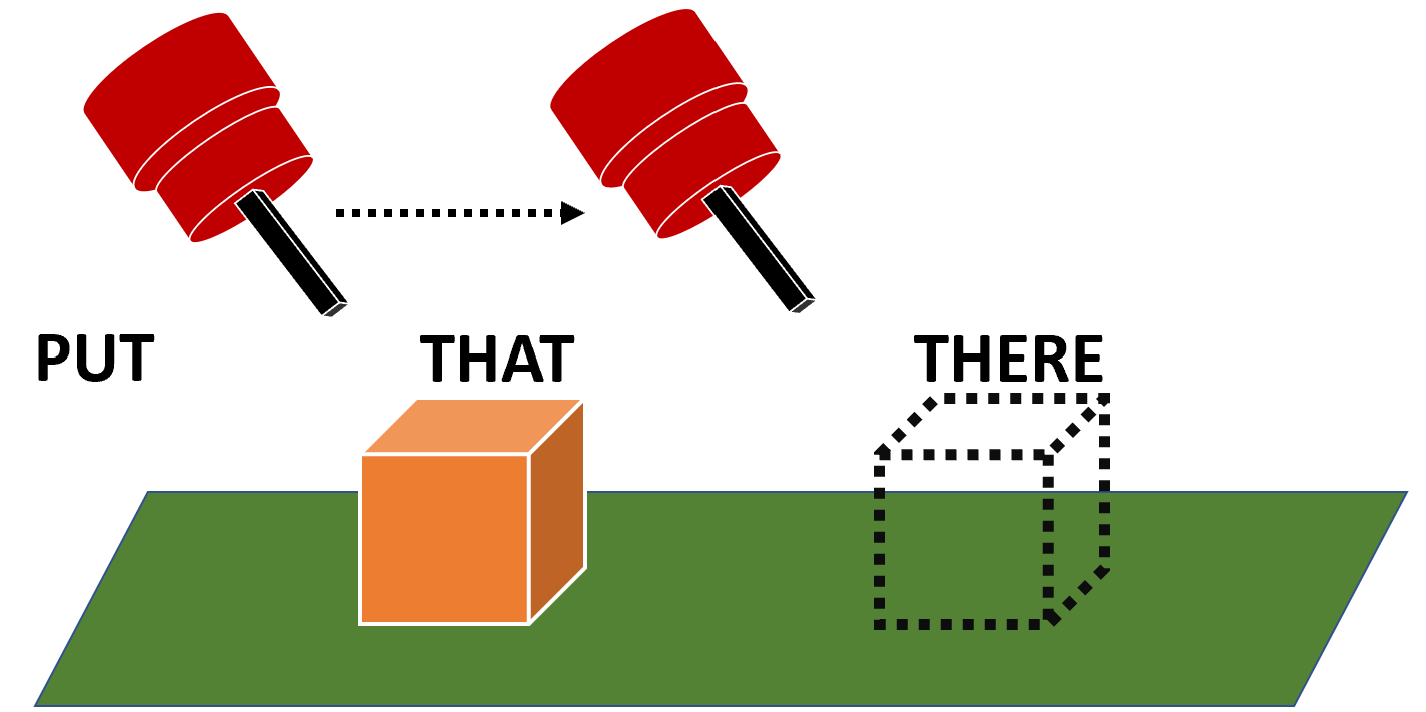
\includegraphics[width=0.4\textwidth, trim={0 0.3in 0 0in},clip]{figures/putthatthere2.png}
    \caption{A pick-and-place task requires a \textit{referential} pointing action to the object (orange cube) at the initial position, and a \textit{locating} pointing action to a final placement position (dotted cube). Such an action by a robot (in red) can also be accompanied by verbal cues like \textit{"Put that there."}}
    \label{fig:pap}
\end{figure}

The second contribution is a set of interpretive principles, inspired by the literature on vague communication, that summarize the above findings about robot pointing.  Our results suggest that pointing selects from a set of candidate interpretations determined by the type of information specified, the possibilities presented by the scene, and the options compatible with the current task.  In particular, we propose that pointing picks out all candidates that are not significantly further from the pointing ray than the closest alternatives.  Based on our empirical results, we present design principles that formalize the relevant notions of ``available alternatives'' and ``significantly further away'' and can be used in implementing future pointing robots.  The Analysis and Design Principles sections explains and justifies this approach and contextualizes it with previous research.

% \malihe{continuous trajectory:


% }

% \malihe{

% -- the reversed task
% In the first set of experiments, the robot is pointing to an area towards the middle part of the table. We point to areas towards the edge of the table to control for this effect, i.e., the pick and place positions of the object are ‘reversed’. The place results provide a balance for the location that the subjects thought the robot was pointing at in the pick trials.

% -- Baxter’s head
% Baxter has a head above the torso. The effect of eye gaze in the interpretation of pointing action in human-human interaction has been studied by cognitive scientists. We acknowledge that it is an important factor. For this paper, however, we are not experimenting with this aspect. We are not using eye gaze and head position is fixed. Another important motivating reason to not rely on eye-gaze can be demonstrated by the second Kuka arm which has no such head. Such a ‘head’ is not a general feature of robotic manipulators and we chose to not focus on eye-gaze effects as a part of the current study.
% }





% Communication is anchored to the material world, to space, to events and people. One way it gets anchored is through pointing. 

Enabling robots to understand and generate instructions to collaboratively solve tasks with humans is an active area of research in natural language processing and human-robot interaction, see \cite{cha2018survey,butepage2017human} for review.   We focus here specifically on research that looks at the role of pointing gestures in communication.

Initial efforts in robotics have looked at making pointing gestures legible, adapting the process of motion planning so that robot movements are correctly understood as being directed toward the location of a particular object in space \cite{holladay2014legible,zhao2016experimental}.  Our work uses motions that are legible in this sense, and goes on to explore how precise the targeting has to be to signal an intended interpretation.

In natural language processing research, it's common to use an expanded pointing cone to describe the possible target objects for a pointing gesture, based on findings about human pointing \cite{kranstedt2003deixis,rieser2004pointing}.  In cluttered scenes, the pointing cone typically includes a region with many candidate referents.  Understanding and generating object references in these situations involves combining pointing with natural language descriptions \cite{han2018placing,kollar2014grounding}.  While we also find that many pointing gestures are ambiguous and can benefit from linguistic supplementation, our results challenge the assumption of a uniform pointing cone; we argue for an alternative, context-sensitive model.

In addition to gestures that identify objects, we also look at pointing gestures that identify points in space.  The closest related work involves navigation tasks, where pointing can be used discriminate direction (e.g., left vs right) \cite{mei2016listen,tellex2011understanding}.  The spatial information needed for pick-and-place tasks is substantially more precise; our findings suggest that this precision has far-reaching implications for how pointing is interpreted and how it should be modeled.



% Notes:
% Robotics: describe a cost function that you can plug into your motion generation. They point to an object and move towards it they have a very rigid cost function that exaggerates the ray...

% NLP people use a more flexible model of pointing to objects-- the pointing cone. They study cluttered scenes where the pointing cone includes several objects on the table. They use the cone basically to point to an area on the table and then they disambiguate using both natural language commands and 
% eye gaze, the shape of the arm etc.
% They don't look at the difference between objects can affect the interpretation of the pointing action. 
%%%%%%%%%%%%%%%%%

% Roboticists have indentified the importance of pointing actions in the context of conveying the intent of motions generated by robotic manipulators. Legibility was used as a metric to devise cost functions, and generate motions without speech \cite{zhao2016experimental,holladay2014legible}. These studies proposed rigid models that treats the objective of communication of the object a robot is about to pick as one of the optimization criteria. The current work studies the inherent flexibility of vague pointing gestures towards both referent objects and parts of the space, in communicating an entire pick-and-place task.



% In natural language processing, people have studied understanding and generation of multimodal referring expressions. This involves studying the generation of referring expressions together with the pointing action to pick a target referent. For instance,  \cite{kollar2014grounding,han2018placing} have shown how and when natural language is efficient for constructing spatial-semantic representations of known environments. \cite{kennington2013interpreting} proposed a discriminative model of incremental reference resolution. The focus of these studies is on designing models for generating referring expression for a target object. 
% These works do not investigate the difference between the richness of intents that pointing can express that we study in this paper. 
% This is true about cognitive and linguistics studies as well \cite{kita2003pointing,kita2003interplay,clark2003pointing,goodwin2003pointing}.
% Pointing has been the subject of cognitive and linguistics studies as a situated practice \cite{kita2003pointing,kita2003interplay,clark2003pointing,goodwin2003pointing}.
% They have relaxed the model of the pointing ray by introducing the pointing cone. 
% The pointing cone model specifies that the target of pointing action has to fall into the cone that comes out of the pointing finger \cite{rieser2004pointing,kranstedt2003deixis}. These studies do not narrow down a generative process that is necessary in the context of human robot interaction. Moreover, they do not investigate the difference between the richness of intents that pointing can express that we study in this paper.

% Our work however, proposes a new challenge. It considers the problem of a robot performing pointing actions to communicate a pick-and-place task to a human observer. This involves pointing to identify object placement in space which has been mainly overlooked by the previous literature. Furthermore, this work proposes that picking is more flexible compared to the rigid models proposed by prior work. We also study the effects of common ground and perspective on domains of referential interpretation. We present experiments testing our hypothesis. Evaluations on two different robotic arms, which are visually distinct, indicate the applicability of our hypothesis in general robotic pointing tasks.

% These works require a semantically labeled representation of the environment.














\section{Communicating Pick-and-Place}
\label{problem}

This section provides a formalization of pick-and-place tasks and identifies  information required to specify them.
 
\noindent\textbf{Manipulator}: A class robotic systems robots that can physically interact with their surroundings are called \textit{manipulators}, of which robotic arms are the prime example. 

\noindent\textbf{Workspace}: The manipulator operates in a 3D workspace $\mathcal{W} \subseteq \mathbb{R}^3$. The workspace also contains a stable surface of interest defined by a plane $S\subset\mathcal{W}$ along with various objects. To represent 3D coordinates of workspace positions, we use $x\in\mathcal{W}$. 

\noindent\textbf{End-effector}: The \textit{tool-tips} or \textit{end-effectors} are geometries, often attached at the end of a robotic arm, that can interact with objects in the environment. These form a manipulator's chief mode of picking and placing objects of interest and range from articulated fingers to suction cups. A subset of the workspace that the robot can \textit{reach} with its end-effector is called the reachable workspace. The end-effector in this work is used as a pointing indicator.

\noindent\textbf{Pick-and-place}: Given a target object in the workspace, a \textit{pick-and-place} task requires the object to be picked up from its initial position and orientation, and placed at a final position and orientation. When a manipulator executes this task in its reachable workspace, it uses its end-effector. 
The rest of this work ignores the effect of the object's orientation by considering objects with sufficient symmetry. Given this simplification, the pick-and-place task can be viewed as a transition from an initial position $x_{init}\in\mathcal{W}$ to a final placement position $x_{final}\in\mathcal{W}$.  Thus, a pick-and-place task can be specified with a tuple
$$ PAP = < o, x_{init}, x_{final} >. $$


\begin{figure}[t]
    \centering
    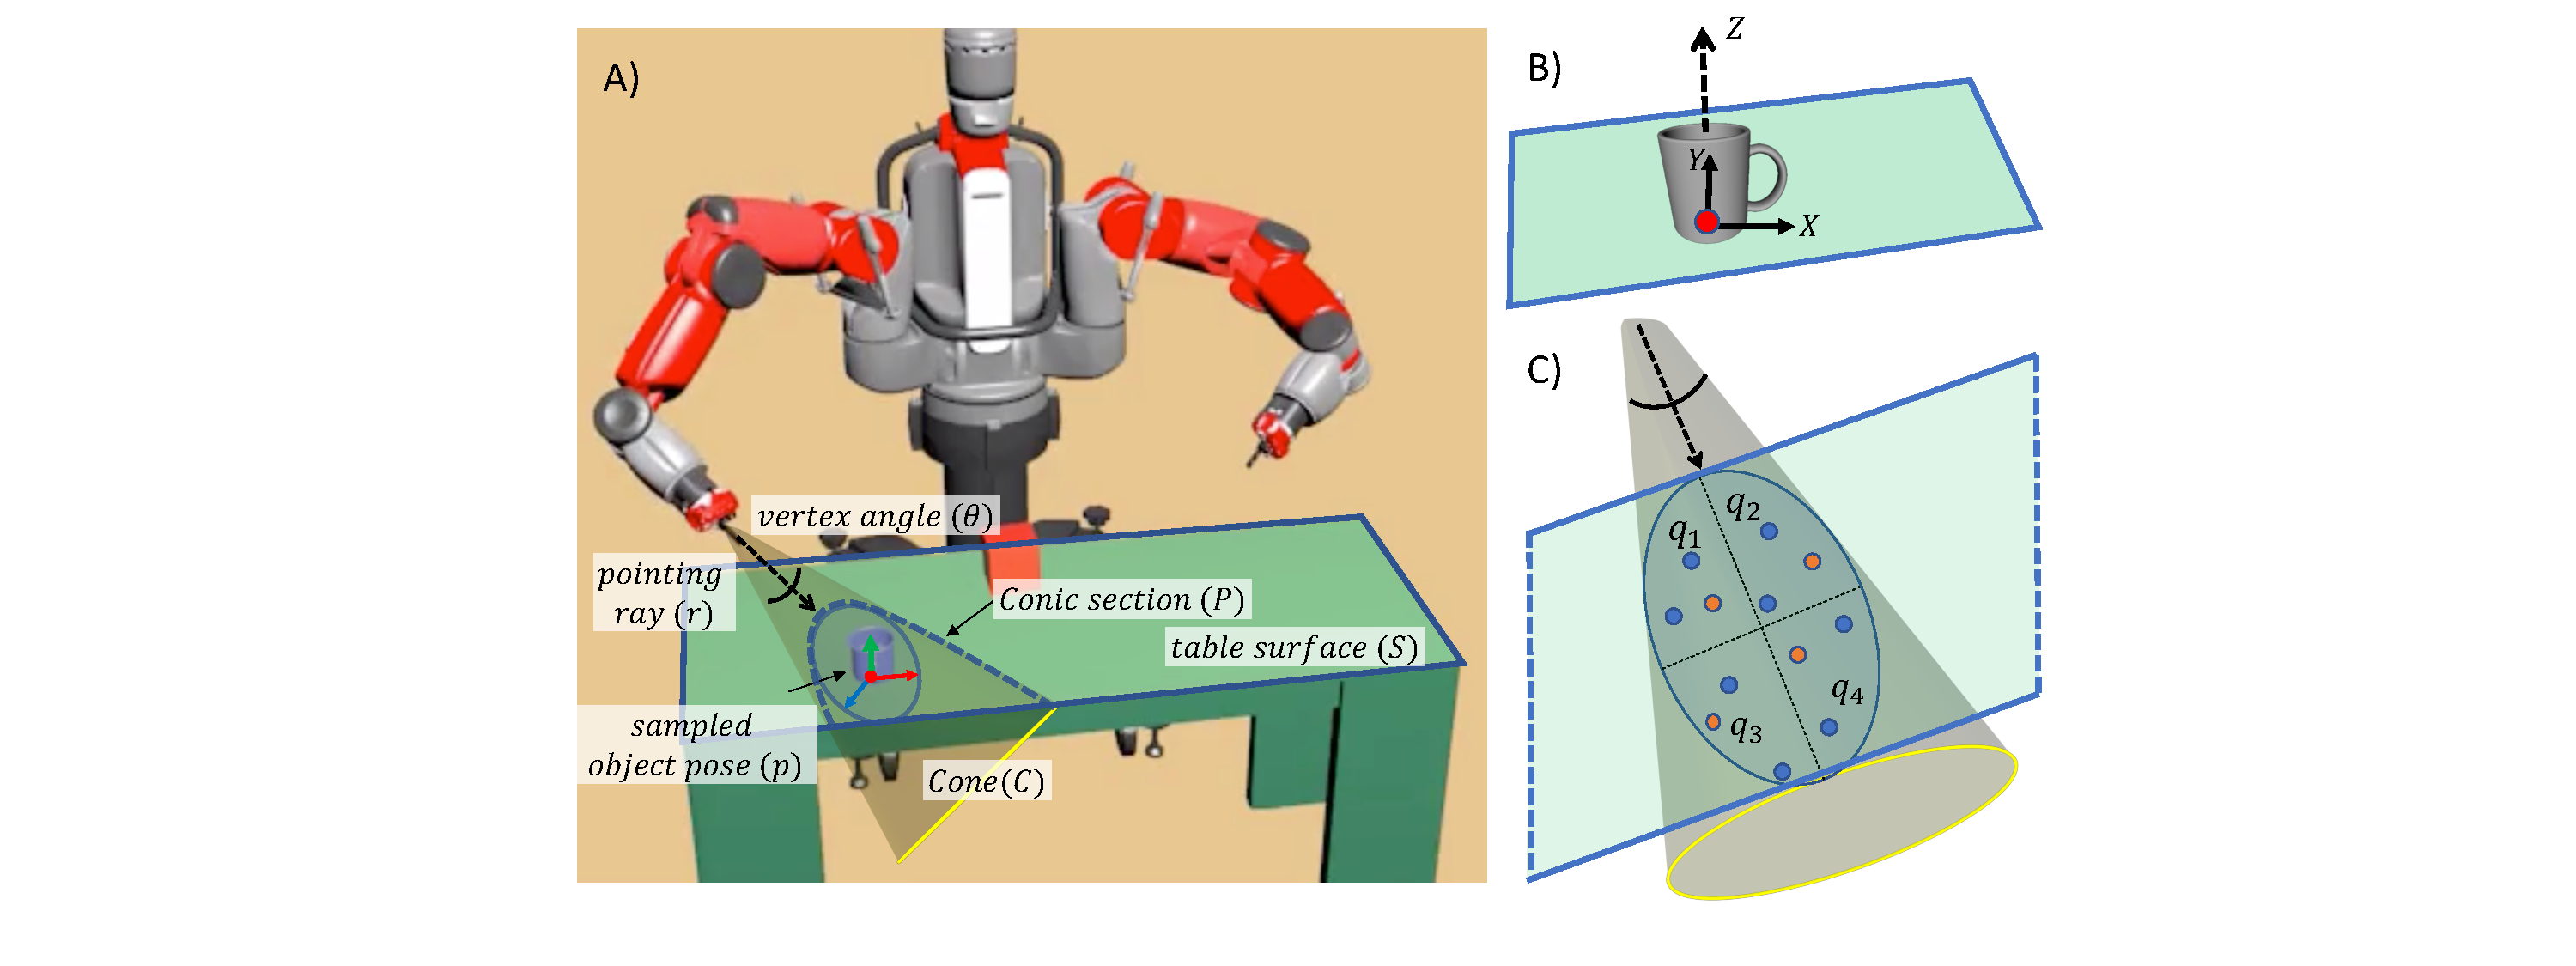
\includegraphics[width=0.5\textwidth]{pointing_diagram}
    \caption{(A) Workspace setup showing the pointing cone and the corresponding conic section on the table. (B) The degrees-of-freedom considered for placement of the object on the table. (C) Sampling policy to sample object poses within the conic section.}
    \label{fig:pointing}
\end{figure}

\noindent\textbf{Pointing Action}: Within its reachable workspace the end-effector of the manipulator can attain different orientations to fully specify a reachable \textit{pose} $p$, which describes its position and orientation.  The robots we study have a directional tooltip that viewers naturally see as projecting a ray $r$ along its axis outward into the scene.  In understanding pointing as communication, the key question is the relationship between the ray $r$ and the spatial values $x_{init}$ and $x_{final}$ that define the pick-and-place task.

% Initially we shall describe this relationship of \textit{pointing} loosely, and narrow down on what it entails through our study.

To make this concrete, we distinguish between the \emph{target} of pointing and the \emph{intent} of pointing. Given the ray $r$ coming out of the end-effector geometry, we define the target of the pointing as the intersection of this ray on the stable surface, $$x^*= r\cap S.$$ Meanwhile, the intent of pointing specifies one component of a pick-and-place task.  There are two cases:
\begin{itemize}
    \item [-] \textit{Referential Pointing:} The pointing action is intended to identify a target object $o$ to be picked up. This object is the \textit{referent} of such an action. We can find $x_{init}$, based on the present position of $o$.
    \item [-] \textit{Locating Pointing:} The pointing action is intended to identify the location in the workspace where the object needs to be placed, i.e, $x_{final}$.
\end{itemize}


We study effective ways to express intent for a pick-and-place task. In other words, what is the relationship between a pointing ray $r$ and the location $x_{init}$ or $x_{final}$ that it is intended to identify?  To assess these relationships, we ask human observers to view animations expressing pick-and-place tasks and classify their interpretations.  To understand the factors involved, we investigate a range of experimental conditions.

% \noindent\textbf{Hypothesis}: One way to model the accuracy of the pointing action is to measure the precision of the focused area of a pointing gesture, the so-called pointing cone. We challenge this argument by identifying two main behaviours: referential pointing and locating pointing.  Our main hypothesis is that the interpretation of pointing actions when the target is part of the space is different from when the target is an object. We expect to run some exploratory studies as well to study how the verbal content and arrangement of objects in the gesture space can influence the interpretation of the pointing action in these two scenarios.


This section first describes the commonalities of the experiments that were designed to test our hypothesis, in terms of the experimental setup. The specific variants of the experiments that were run is described as a part of the methods. 
All of the experiments described in this section together with the methods that we have chosen to analyze the data based on a private but approved pre-registration on \textit{aspredicted.org}. We will make the pre-registration public once the anonymity period ends.

\subsection{Experiment Setup}
The setup of the experiment describes the robots used, the environment with the objects and the procedures to generate motions and actions necessary to design different evaluation conditions.

\noindent\textbf{Robotic Platforms}: The experiments were performed on two separate robotic platforms, a \textit{Rethink Baxter}, and a \textit{Kuka IIWA14}.
The \textit{Baxter} is a dual-arm manipulator with two arms mounted on either side of a static torso. The experiments only move the right arm of the \textit{Baxter}. The \textit{Kuka} is consists of a single arm that is vertically mounted, i.e., points upward at the base. In the experiments the robots are fitted with a singly fingered tooltip, where pointing gestures are designed in terms of the outward ray coming out of the end-effector.



\noindent\textbf{Workspace Setup}: Objects are placed in front of the manipulators. In certain trials a table is placed in front of the robot as well, and the objects rest in stable configurations on top of the table. A pick-and-place task is provided specified in terms of the positions of one of the objects. 

\noindent\textbf{Objects}: The objects used in the study include small household items like mugs, saucers and boxes (cuboids), that are all placed in from on the robots.

\noindent\textbf{Motion Generation}: The end-effector of the manipulator is instructed to move to pre-specified waypoints that typically lie between the base of the manipulator and the object itself. Such waypoints fully specify both the position and orientation of the end-effector to satisfy \textit{pointing actions}. The motions are performed by solving \textit{Inverse-Kinematics} for the end-effector geometry and moving the manipulator along these waypoints using a robotic motion planning library \cite{littlefield2014extensible}. The motions were replayed on the model of the robot, and rendered in \textit{Blender}.

% \begin{figure}[t]
%     \centering
%     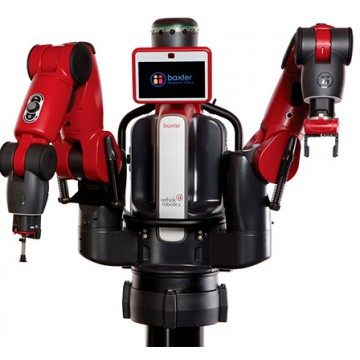
\includegraphics[width=0.23\textwidth]{baxter.jpg}
%     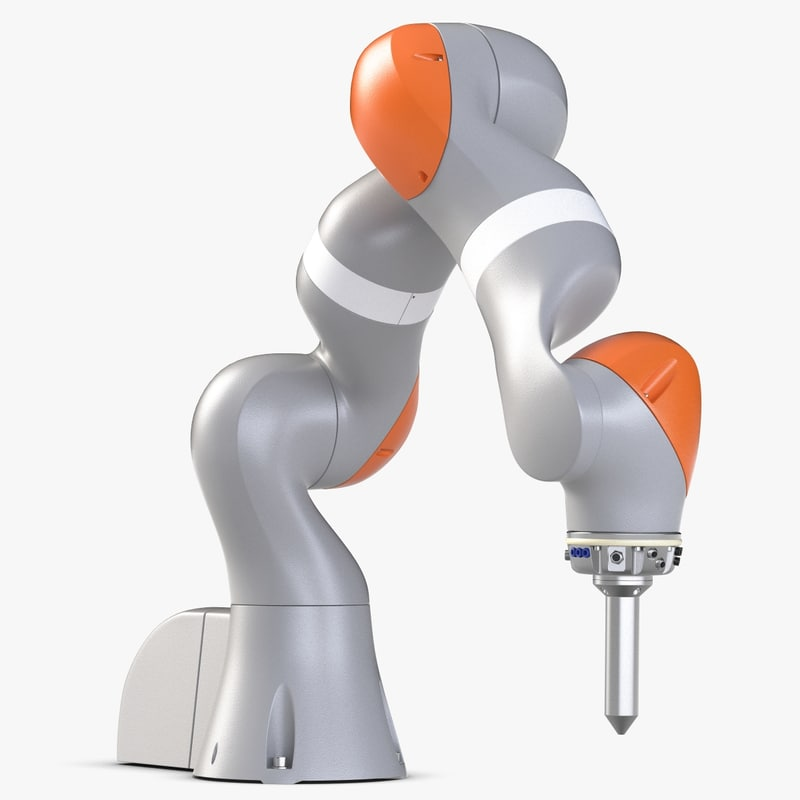
\includegraphics[width=0.23\textwidth]{kuka.jpg}
%     \caption{The robots used in the study are the \textit{Rethink Baxter}(left) and the \textit{Kuka IIWA14}(right)(<references>)}
%     \label{fig:robots}
% \end{figure}

\begin{figure}[th!]
    \centering
    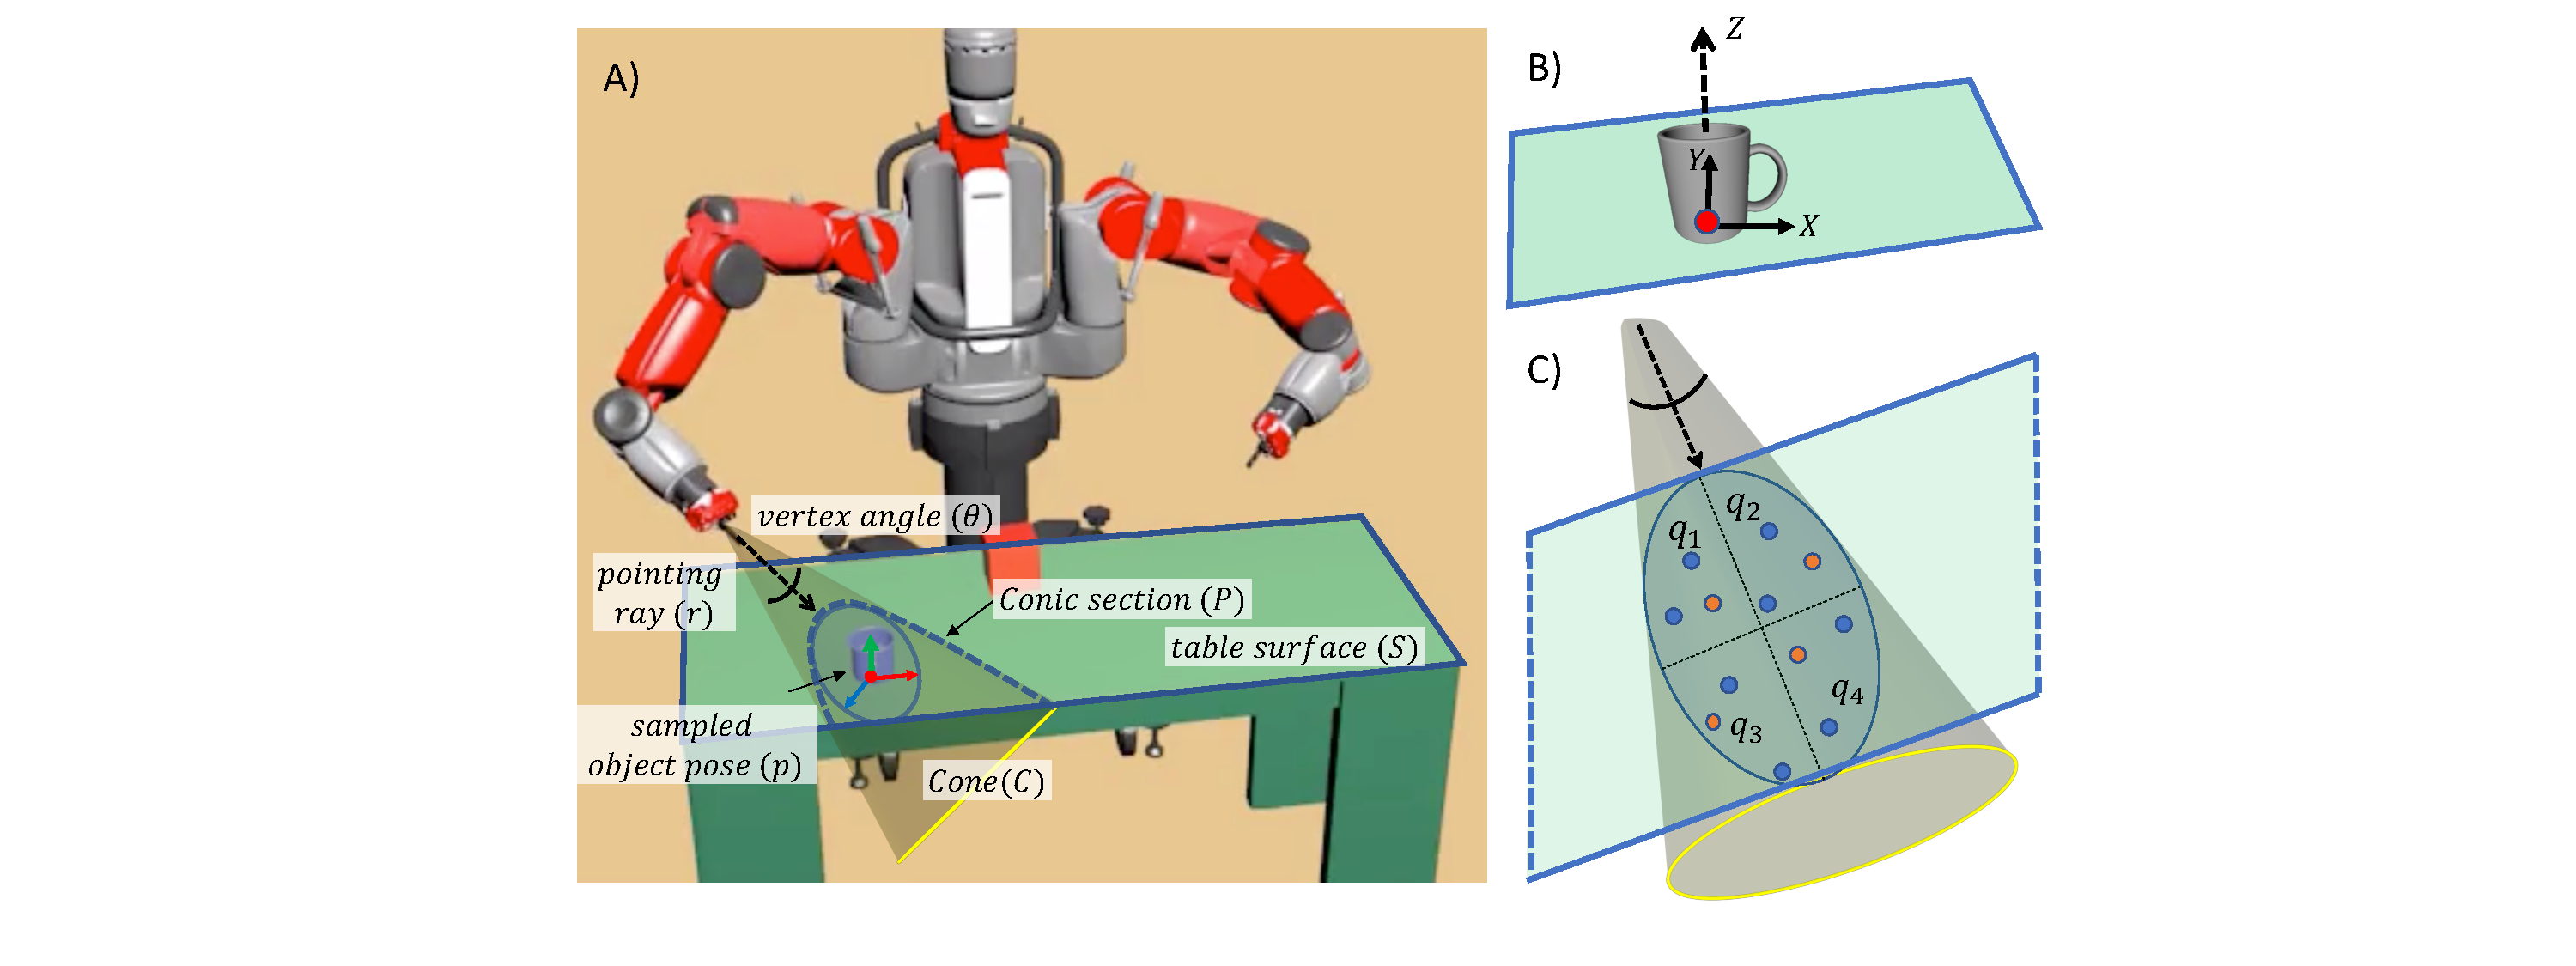
\includegraphics[width=0.5\textwidth]{pointing_diagram}
    \caption{(A) Workspace setup showing the pointing cone and the corresponding conic section on the table. (B) Shows the degrees-of-freedom considered for placement of the object on the table (C) Sampling policy to sample object poses within the conic section.}
    \label{fig:pointing}
\end{figure}

\begin{figure}[h!]
    \centering
    % 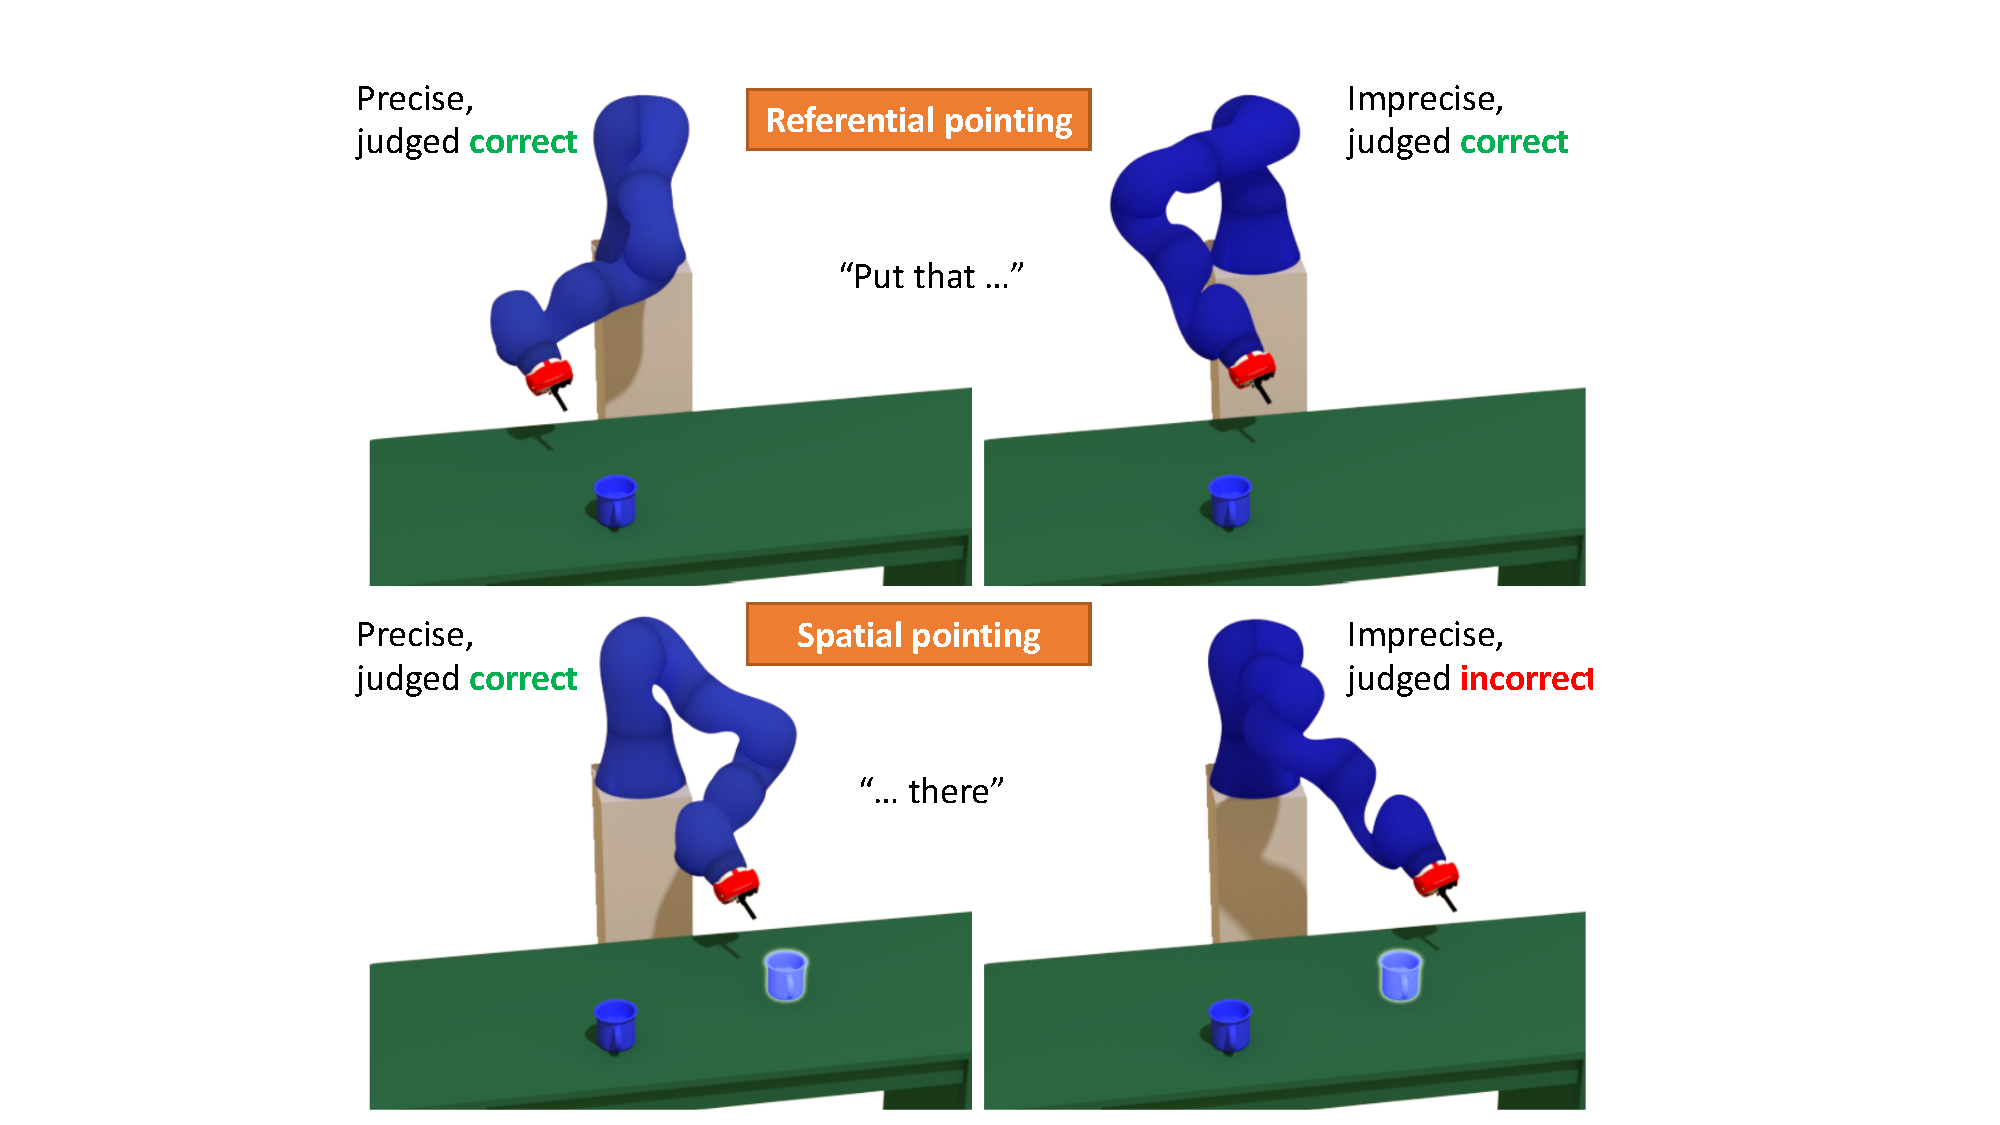
\includegraphics[width=0.5\textwidth]{spatial-referential.pdf}
    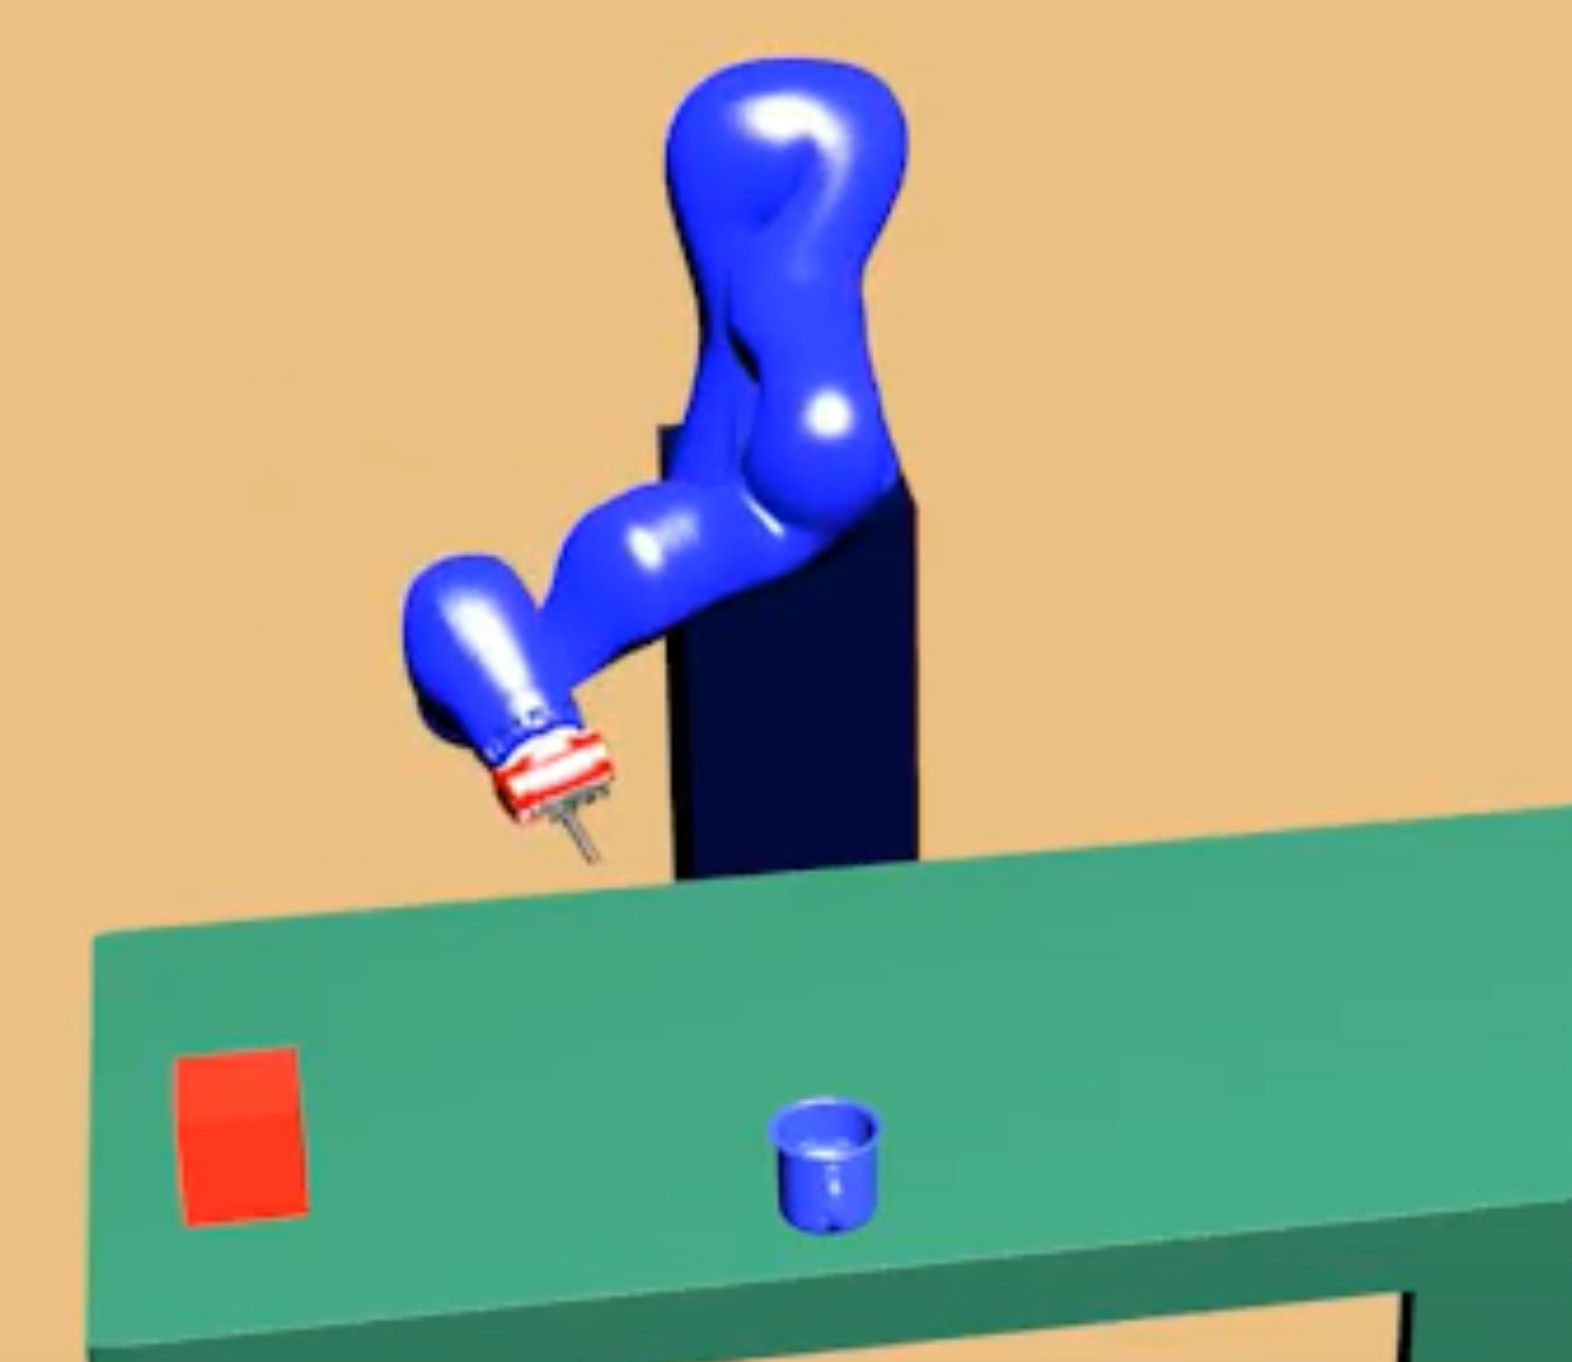
\includegraphics[height=0.20\textwidth]{figures/kuka_ref.png}
    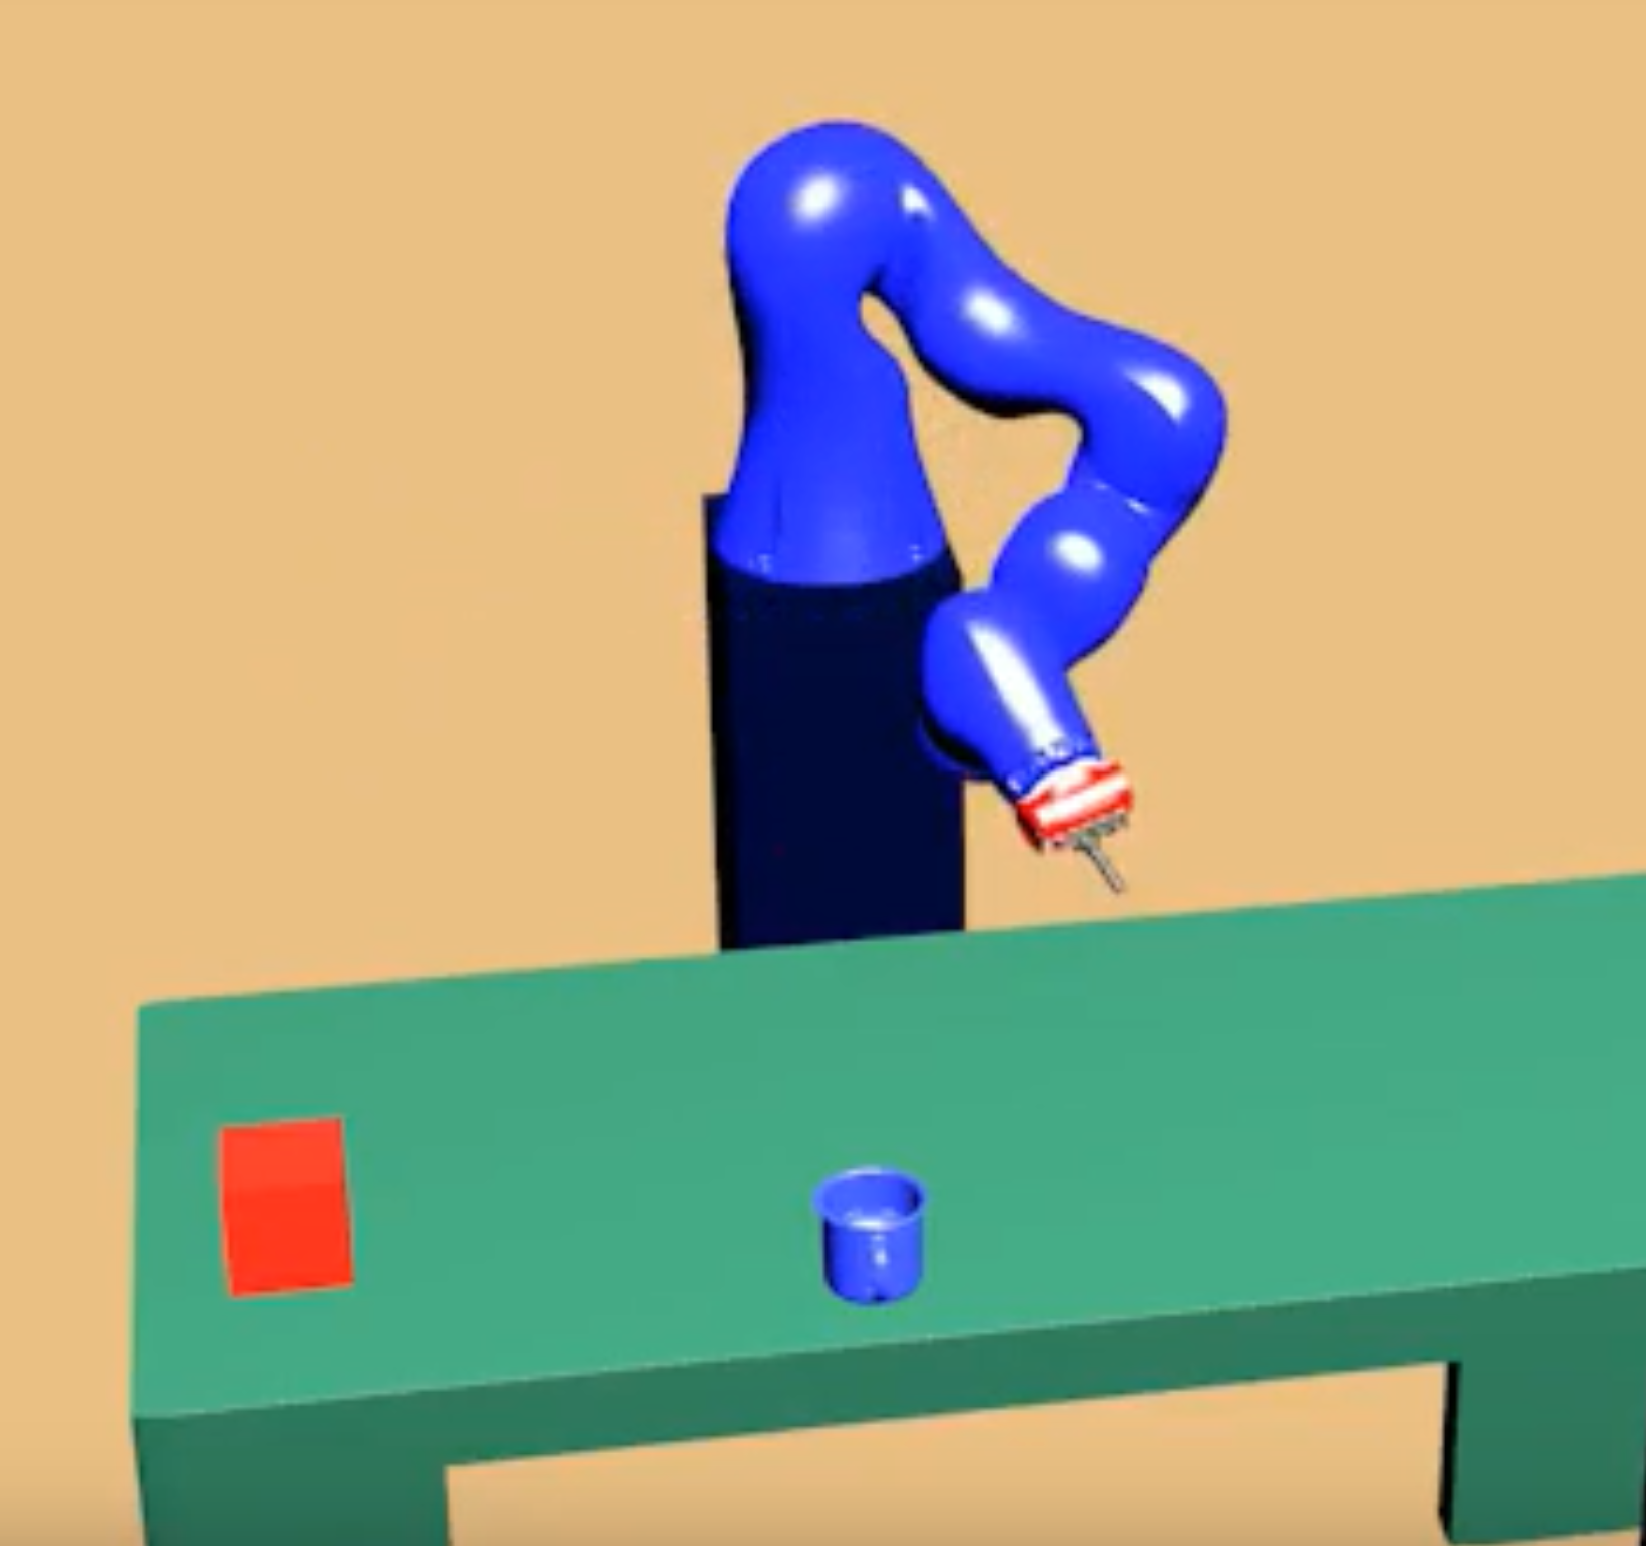
\includegraphics[height=0.20\textwidth]{figures/kuka_spatial.png}
    \caption{Scenes from the simulated setup showing the differences between referential (\textit{left}) and spacial pointing (\textit{right}), demonstrated on a second robotic manipulator, \textit{Kuka IIWA14}.}
    \label{fig:spatial}
\end{figure}

\begin{figure}[h!]
    \centering
    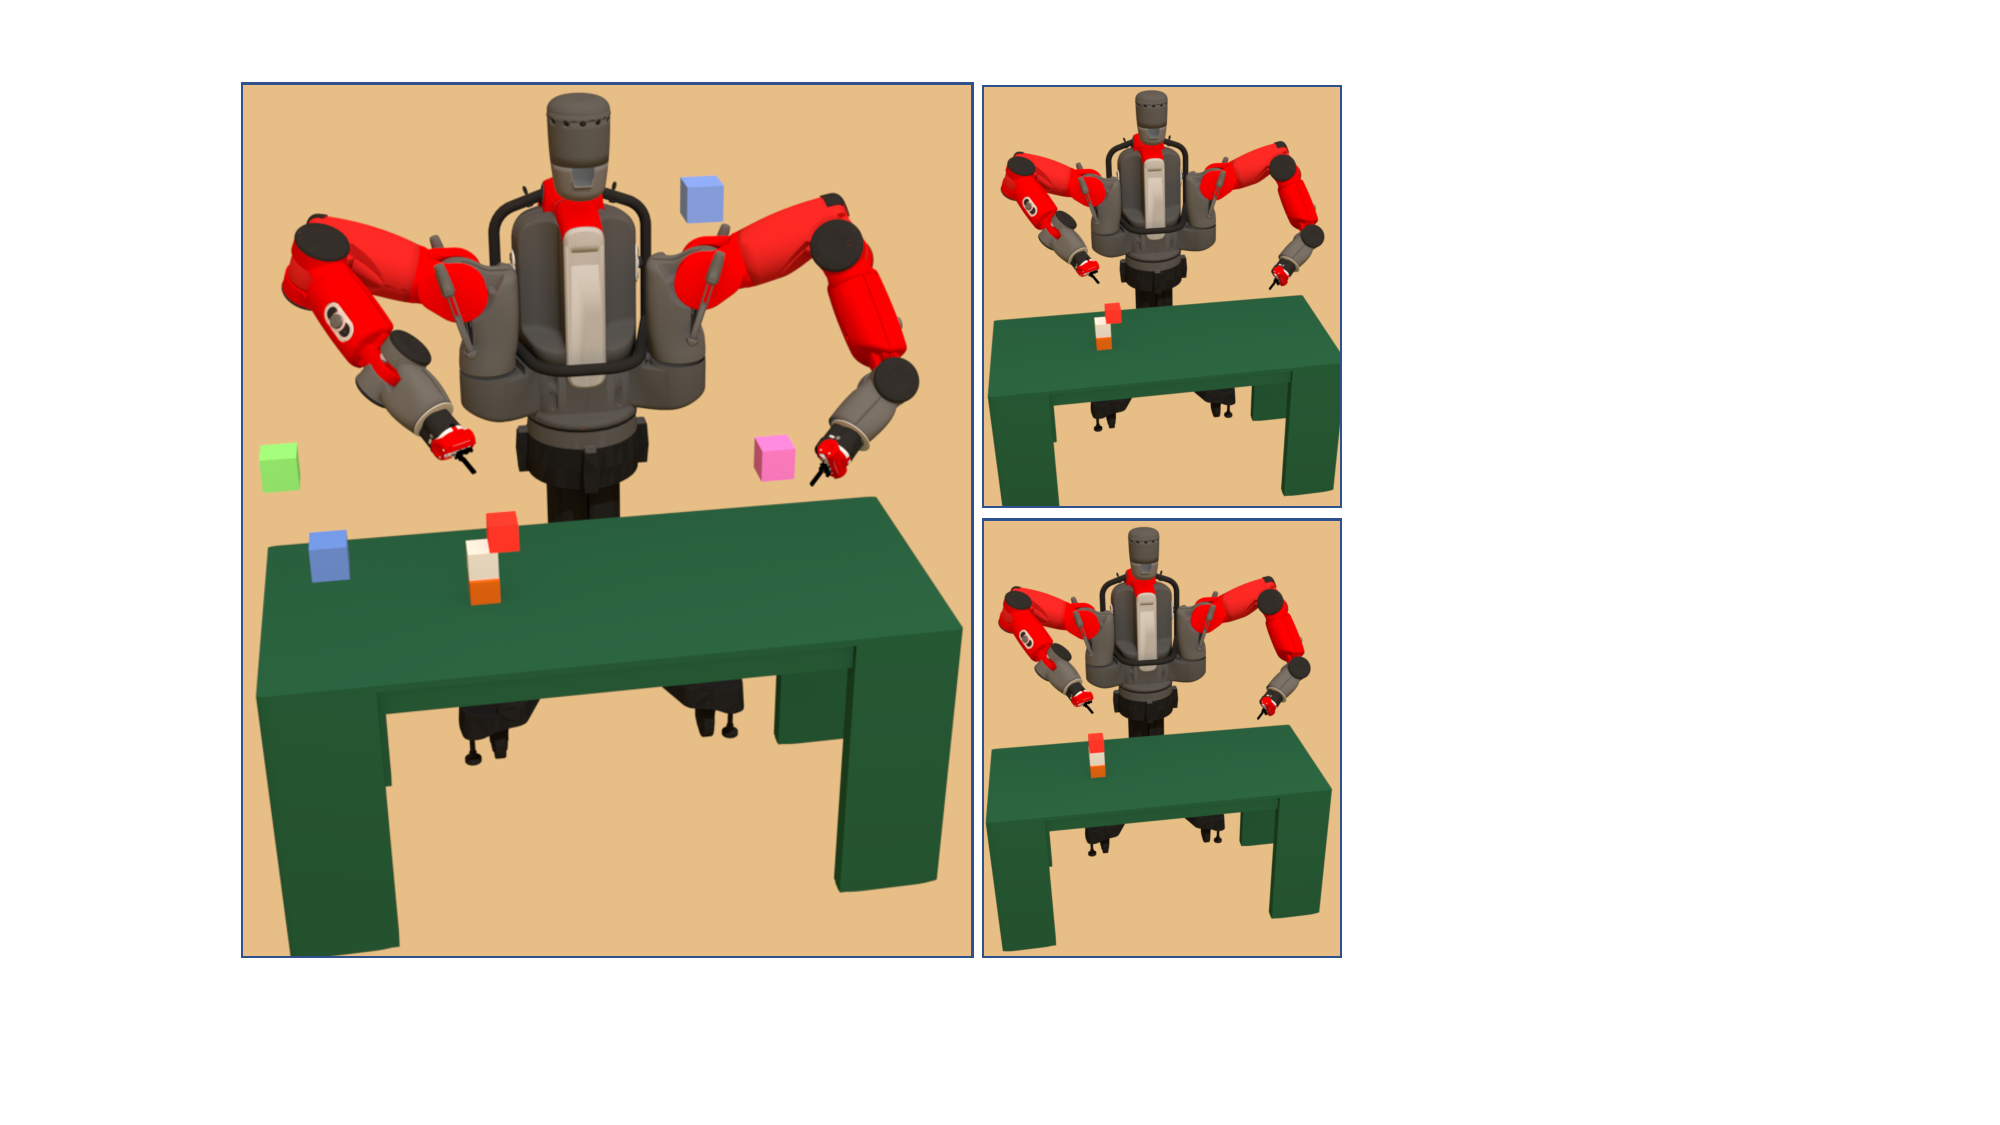
\includegraphics[width=0.45\textwidth]{natural.pdf}
    \caption{(Left) In an unnatural scene, a gesture pointing to an unstable position (edge of the stack) is deemed correct. (Right) In natural scenes, although the robot points to the edge of the stack, a physically realistic object position gets more user vote than the unstable position.}
    \label{fig:natural}
\end{figure}

% \noindent\textbf{Pointing Action Generation}: Pointing gesture is modeled by a cone $C(r, \theta)$ coming out of the pointing finger where $r$ represents the axis and $\theta$ represents the vertex angle of the cone. As illustrated in Fig~\ref{fig:pointing}, a robot is using it's finger to point to an object placed on a rest surface. For the scope of this study we assume that the rest surface is a plane represented by $S$. Thus the conic section formed on the surface of the table is given by $P=C \cap S$.

% To identify the geometry for the correct pointing gesture in different cases, $N$ object poses $p_i, i=1:N$ are sampled within the conic section $P$. While $p_i$ is the 6d pose for the object with translation $t \in R^3$ and orientation $R \in SO(3)$ only 3 degrees-of-freedom $(x, y, yaw)$ are varied for the experiments. By fixing the $z$ coordinate and the z-axis of rotation, it is ensured that the object rests in a physically stable configuration on the table.

% To sample $N$ poses, the largest eclipse that fits into the conic section $P$ is divided into 4 quadrants $q_1:q_4$ (See Figure~\ref{fig:pointing} (C)) . Within each quadrant $q_i$ the $N/4$ $(x,y)$ positions are sampled uniformly at random. For each placement $yaw$ is randomly sampled from the domain $(0, 2\pi)$. 

\noindent\textbf{Pointing Action Generation}: Pointing gesture is modeled by a cone $C(r, \theta)$ coming out of the pointing finger where $r$ represents the axis and $\theta$ represents the vertex angle of the cone. As illustrated in Fig~\ref{fig:pointing}, a robot is using it's finger to point to an object placed on a rest surface. For the scope of this study we assume that the rest surface is a plane represented by $S$. The part of the conic section that lies on the surface of the table is given by $P=C \cap S$.

To identify the geometry for the correct pointing gesture in different cases, $N$ object poses $p_i, i=1:N$ are sampled within $P$. While $p_i$ is the 6d pose for the object with translation $t \in R^3$ and orientation $R \in SO(3)$ only 2  degrees-of-freedom $(x, y)$ corresponding to $t$ are varied in the experiments. By fixing the $z$ coordinate for translation and restricting the z-axis of rotation to be perpendicular to $S$, it is ensured that the object rests in a physically stable configuration on the table.

The $N$ object poses are sampled by fitting an ellipse within $P$ and dividing the ellipse into 4 quadrants $q_1:q_4$ (See Figure~\ref{fig:pointing} (C)) . Within each quadrant $q_i$ the $N/4$ $(x,y)$ positions are sampled uniformly at random. For certain experiments additional samples are generated with an objective to increase coverage of samples within the ellipse by utilizing a dispersion measure.

% Malihe needs to check this.


\noindent\textbf{Speech}: Some experiments also included verbal cues with phrases like '\textit{Put that there}' along with the pointing actions. It was very important for the pointing actions and these verbal cues to be in synchronization. To fulfill this we generate the voice using Amazon Polly with text written in SSML format and make sure that peak of the gesture (the moment a gesture comes to a stop) is in alignment with the peak of each audio phrase in the verbal cue. During the generation of the video itself we took note of the peak moments of the gestures and then manipulated the duration between peaks of the audio using SSML to match them with gesture peaks after analyzing the audio with an open-source tool- PRAAT \footnote{www.praat.org}.


\subsection{Experiment Design}

Using the setup of the experiments, videos and images from simulation are generated for different benchmarks, and data is collected to study the differences between the pointing gestures, and test our hypothesis. It should be noted that the restrictions of the a simulated 2D interface of videos, and images, that serve as the form of interaction with human subjects can introduce artifacts of the effect of perspective, which we have attempted to control for.  

\subsection{Data Collection}


Participants are asked to report judgments on the interpretation of the pointing action in each class; referential and spatial.  Each participant undertakes two trials from each class. We introduce a dataset of over 5130 responses to robot pointing actions in this study.

Data collection was performed in \textit{Amazon Mechanical Turk}.
All subjects agreed to a consent form and were compensated at an estimated rate of \textit{USD 20} an hour. The subject-pool was restricted to non-colorblind US citizens. Subjects are presented a rendered video of the simulation where the robot performs one referential pointing action, and one spatial pointing action which amounts to it pointing to an object, and then to a final location. During these executions synchronized speech is included in some of the trials to provide verbal cues.

Then on the same page, subjects see the image that shows the result of the pointing action. They are asked whether the result is (a) correct, (b) incorrect, or (c) ambiguous.  



\subsection{Methods}

To test our hypothesis, we studied the interpretation of the two pointing behaviours in different contexts. Assuming our conjecture and a significance level of 0.05, a sample of 28 people in each condition is enough to detect our effect with a 95\% power.

\paragraph{Referential vs Spatial}
In this trial, to reduce the chances of possible ambiguities, we place only one mug is on the table. The \textit{Baxter} robot points its right arm to the mug and then points to its final position, accompanied by a synchronized verbal cue, '\textit{Put that there.}'

% The final image then presents the accurate final position of the mug. Here, we vary the initial position of the mug that is we sample 8 random points from the three cones explained in section yyy. 

We keep the motion identical across all the trials in this method. 
We introduce a variability in the initial position of the mug by sampling $8$ random positions within conic sections subtending $45^{\circ} , 67.5^{\circ}, $ and $90^{\circ}$, on the surface of the table. New videos are generated for each such position of the mug.
This way we can measure how flexible subjects are to the variation of the initial location of the referent object. 

To test the effect for the spatial pointing action, we test similarly sampled positions around the final pointed location, and display these realizations of the mug as the result images to subjects, while the initial position of the mug is kept perfectly situated. 

 A red cube that is in the gesture space of the robot, and is about twice as big as the mug is placed on the other side of the table as a visual guide for the subjects to see how objects can be placed on the table. 

\noindent\textit{Effect of speech}: In order to test the effect of speech on the disparity between the kinds of pointing actions, a set of experiments were designed under the \textit{Referential vs Spatial} method with and without any speech. All subsequent methods will include verbal cues during their action execution. These cues are audible in the video.


\noindent\textit{Reverse Task}: 

One set of experiments are run for the pick-and-place task with the initial and final positions of the object flipped for the reverse task. This trial is designed to be identical the Referential vs Spatial trials, except for the direction. The motions are still executed on the \textit{Baxter's} right arm. 


\noindent\textit{Different Robotic Arm}:
In order to ensure that the results obtained in this study are not dependent on the choice of the robotic platform or its visual appearance, a second robot - a singly armed industrial \textit{Kuka} manipulator - is evaluated in the Referential vs Spatial study (shown in Figure~\ref{fig:spatial}).

\begin{figure}[t]
    % \vspace{-0.1in}
    \centering
    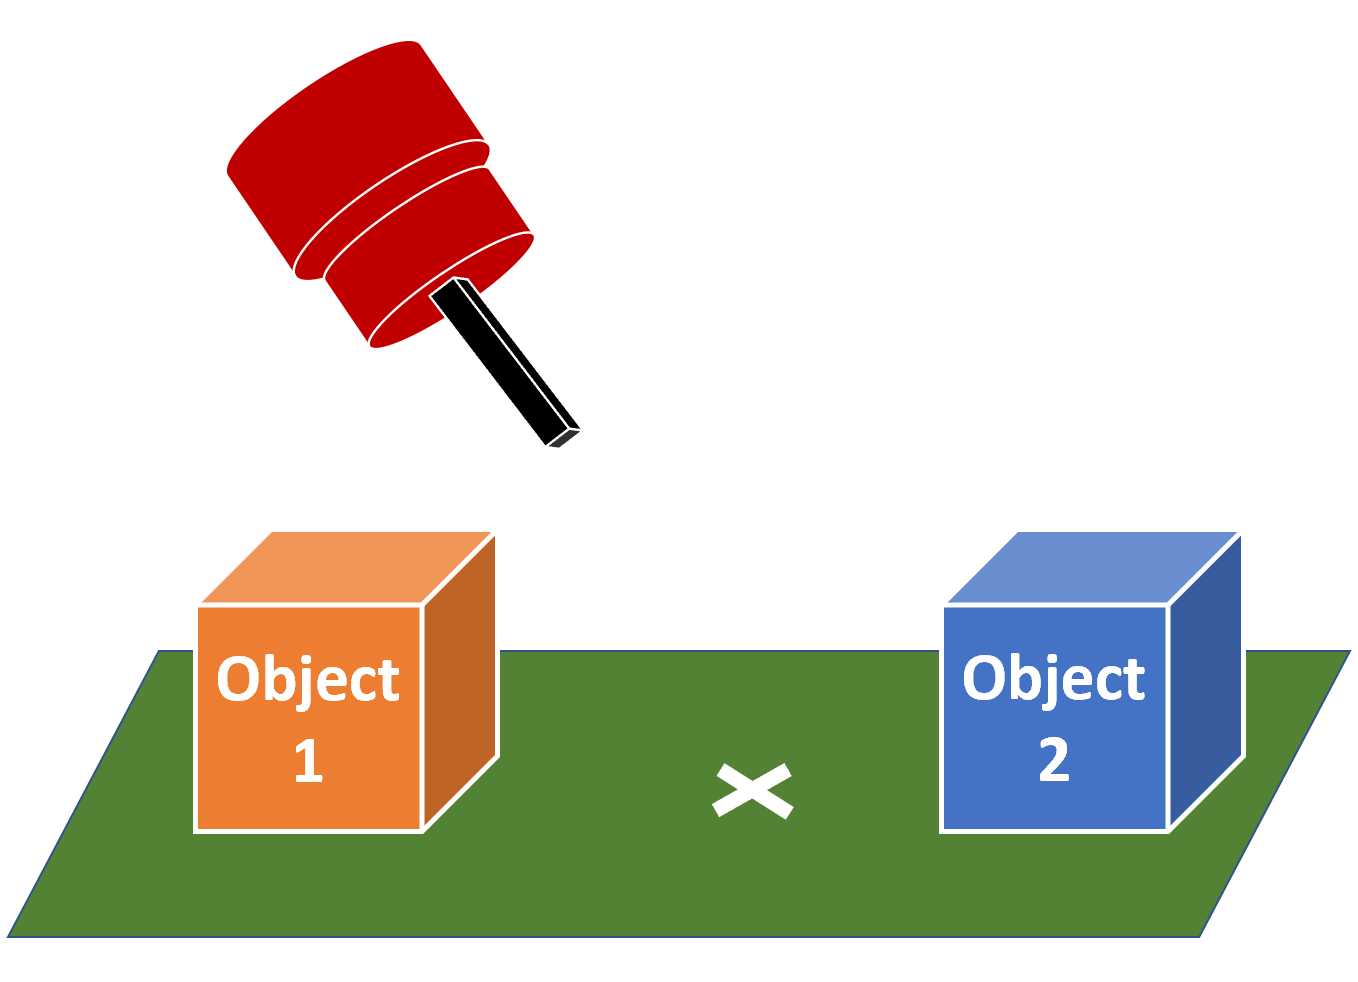
\includegraphics[width=0.3\textwidth]{figures/clutter_trial.png}
    \caption{A cluttered trial consists of collecting the response from a human subject when the position of the referential pointing action lies between two objects.}
    % \vspace{-0.3in}
    \label{fig:cluttered_trial}
\end{figure}
\paragraph{Cluttered Scene}
To study how the presence of other objects would change the behaviour of referential pointing, we examine the interpretation of the pointing actions when there are multiple objects on the tables. We start with a setup where there are 2 cups placed on the table (similar to the setup in Figure~\ref{fig:cluttered_trial}). One is a target cup placed at position $x_{object}$ and a distractor cup at position $x_{distractor}$. With the robot performing an initial pointing action to a position $x_{init}$ on the table. Both the objects are sampled around $x_{init}$ along the diametric line of the conic section arising from increasing cone angles of $45^\circ, 67.5^\circ, $ and $90^\circ$, where the separation of $x_{object}$, and $x_{distractor}$ is equal to the length of the diameter of the conic section, $D$. The objects are then positioned on the diametric line with a random offset between $[-\frac{D}{2}, \frac{D}{2}]$ around $x_{init}$ and along the line. This means that the objects are at various distances apart, and depending upon the offset, one of the objects is nearer to the pointing action. The setup induces that the nearer cup serves as the \textit{object}, and the farther one serves as the \textit{distractor}. The motions are performed on the \textit{Baxter's} right arm. The camera perspective in simulation is set to be facing into the pointing direction. The subjects in this trial are shown images of the instant of the referential pointing action.




\paragraph{Natural vs Unnatural scene}
In this experiment we study how the contextual and physical understanding of the world impacts the interpretation of pointing gestures. We generate a scenario for spatial pointing in which the right arm of the \textit{Baxter} points to a final placement position for the cuboidal object on top of a stack of cuboidal objects but towards the edge which makes it physically unstable. The final configurations of the object (Figure~\ref{fig:topedgetable}) shown to the users were a) object lying on top of the stack b) object in the unstable configuration towards the edge of the stack and c) object at the bottom of the stack towards one side. New videos are generated for each scenario along with verbal cues.

The pointing action, as well as the objects of interest stay the identical between the natural, and unnatural trials. The difference lies in other objects in the scene that could defy gravity and float in the unnatural trials. The subjects were given a text-based instruction at the beginning of an unnatural trial saying they were seeing a scene where "gravity does not exist". 


% \begin{figure*}[t]
%     \centering
%     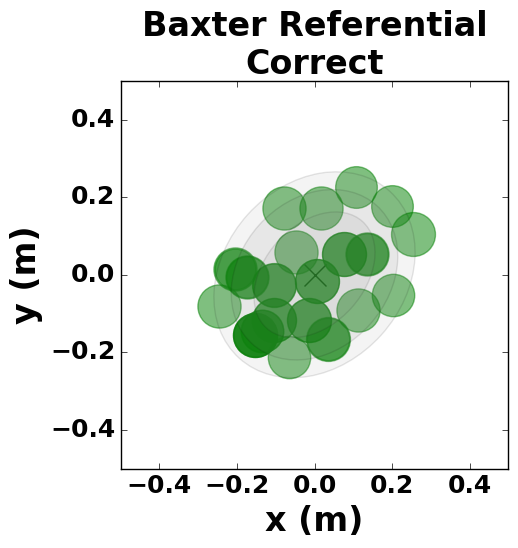
\includegraphics[width=0.32\textwidth ] {figures/baxter_Referential_Correct.png}
%     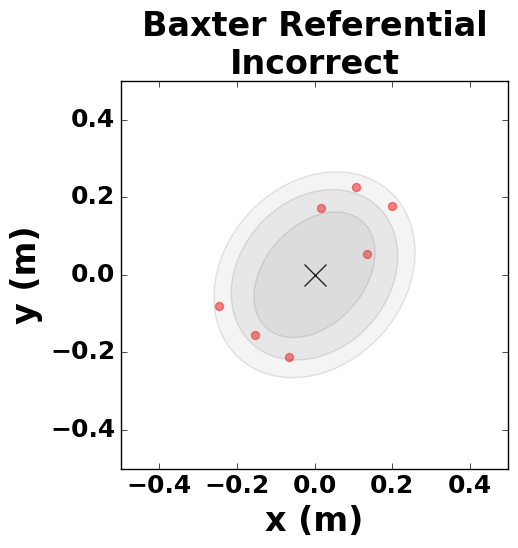
\includegraphics[width=0.32\textwidth ]{figures/baxter_Referential_Incorrect.png}
%     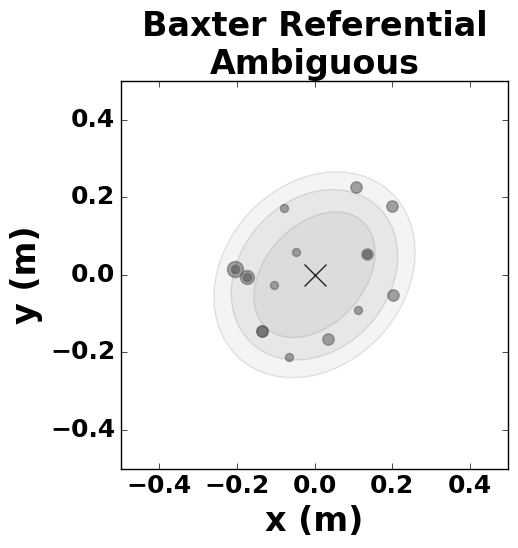
\includegraphics[width=0.32\textwidth ]{figures/baxter_Referential_Ambiguous.png}
%     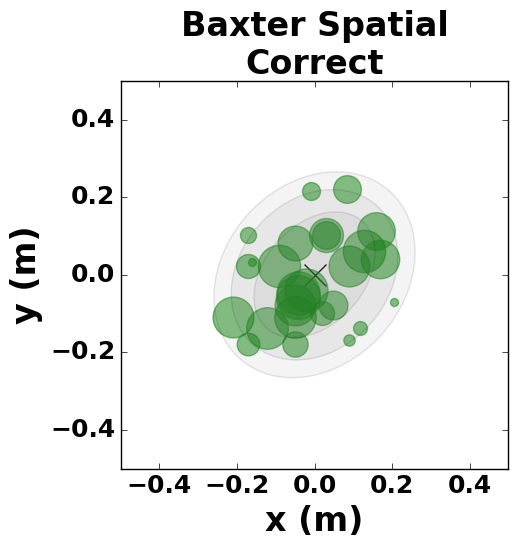
\includegraphics[width=0.32\textwidth ]{figures/baxter_Spatial_Correct.png}
%     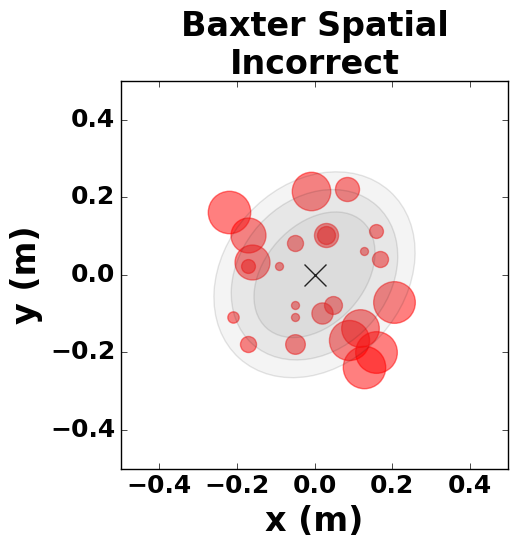
\includegraphics[width=0.32\textwidth ]{figures/baxter_Spatial_Incorrect.png}
%     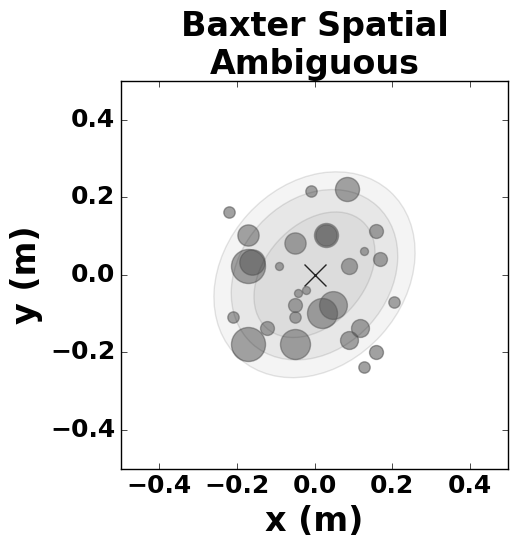
\includegraphics[width=0.32\textwidth ]{figures/baxter_Spatial_Ambiguous.png}
%     \caption{The results from the referential versus spatial trials for the \textit{Baxter} robot. The locations of the responses correspond to the center of the circles, and are plotted in the coordinate frame centered at the position of the true pointing action, marked with $\times$. The size of the circles are proportional to the number of the responses.}
%     \label{fig:baxtersimple}
% \end{figure*}


% \begin{figure*}[t]
%     \centering
%     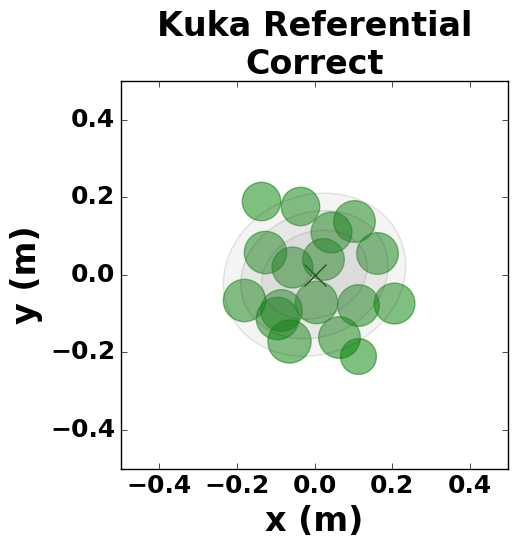
\includegraphics[width=0.32\textwidth ] {figures/kuka_Referential_Correct.png}
%     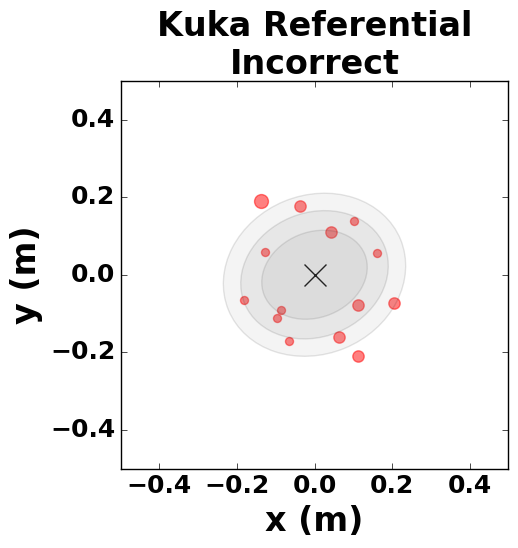
\includegraphics[width=0.32\textwidth ]{figures/kuka_Referential_Incorrect.png}
%     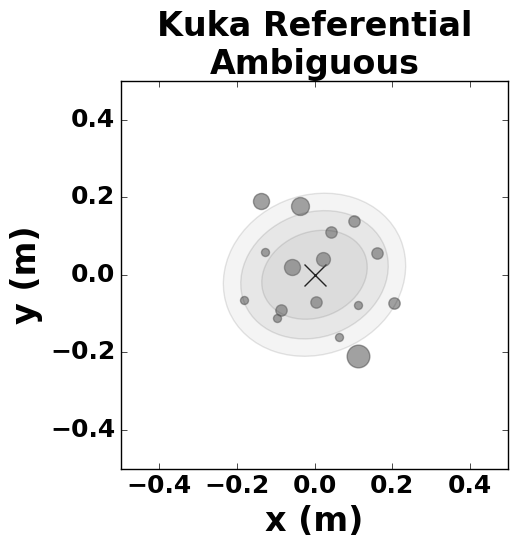
\includegraphics[width=0.32\textwidth ]{figures/kuka_Referential_Ambiguous.png}
%     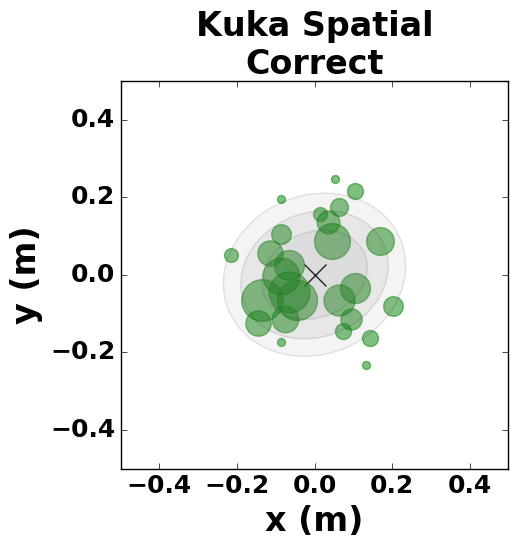
\includegraphics[width=0.32\textwidth ]{figures/kuka_Spatial_Correct.png}
%     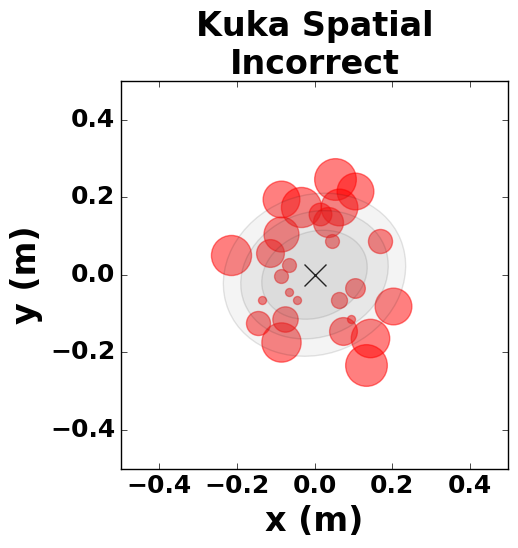
\includegraphics[width=0.32\textwidth ]{figures/kuka_Spatial_Incorrect.png}
%     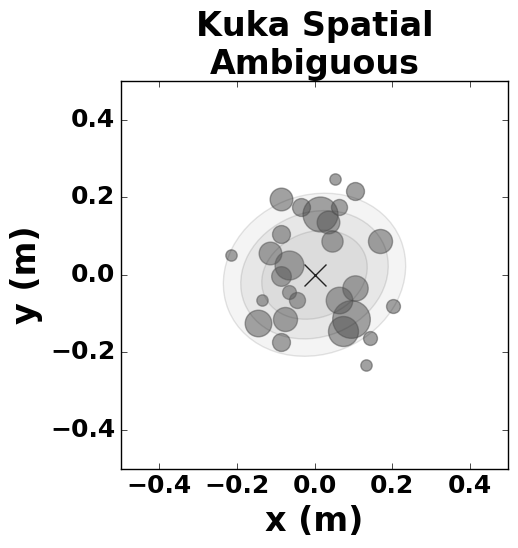
\includegraphics[width=0.32\textwidth ]{figures/kuka_Spatial_Ambiguous.png}
%     \caption{The results from the referential versus spatial trials for the \textit{Kuka} robot. The locations of the responses correspond to the center of the circles, and are plotted in the coordinate frame centered at the position of the true pointing action, marked with $\times$. The size of the circles are proportional to the number of the responses.}
%     \label{fig:kukasimple}
% \end{figure*}



% \begin{figure*}[t]
%     \centering
%     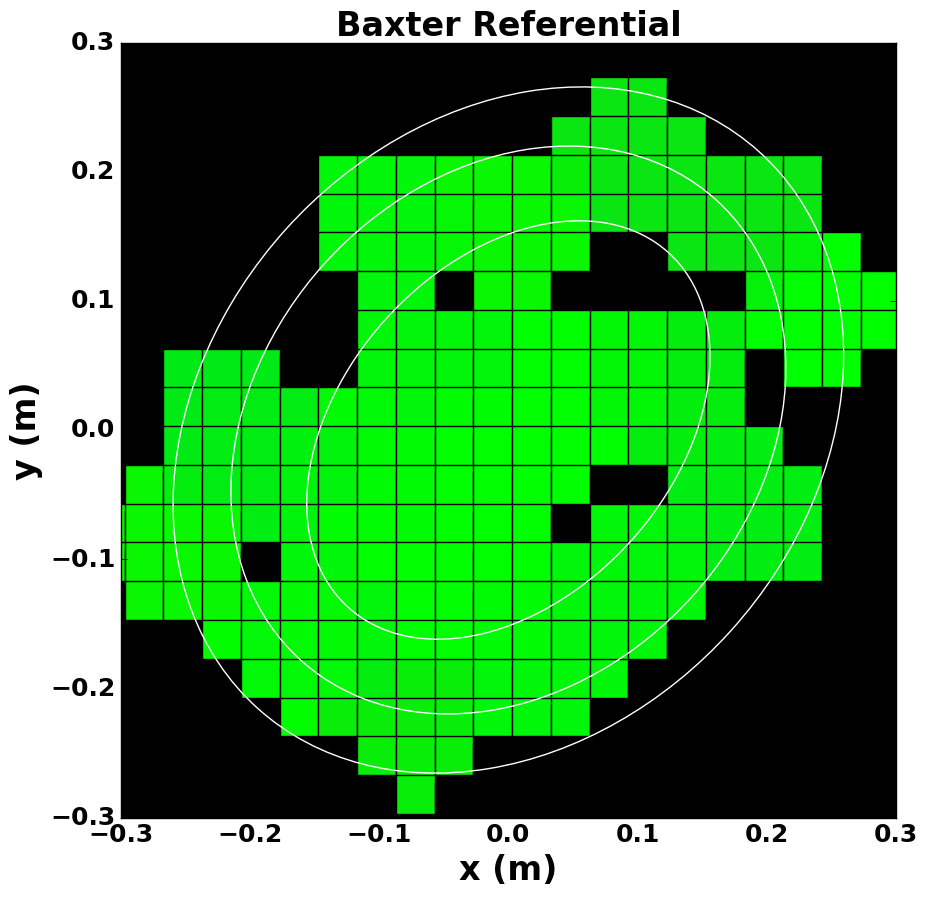
\includegraphics[width=0.4\textwidth ] {figures/baxter_Referential__color.png}
%     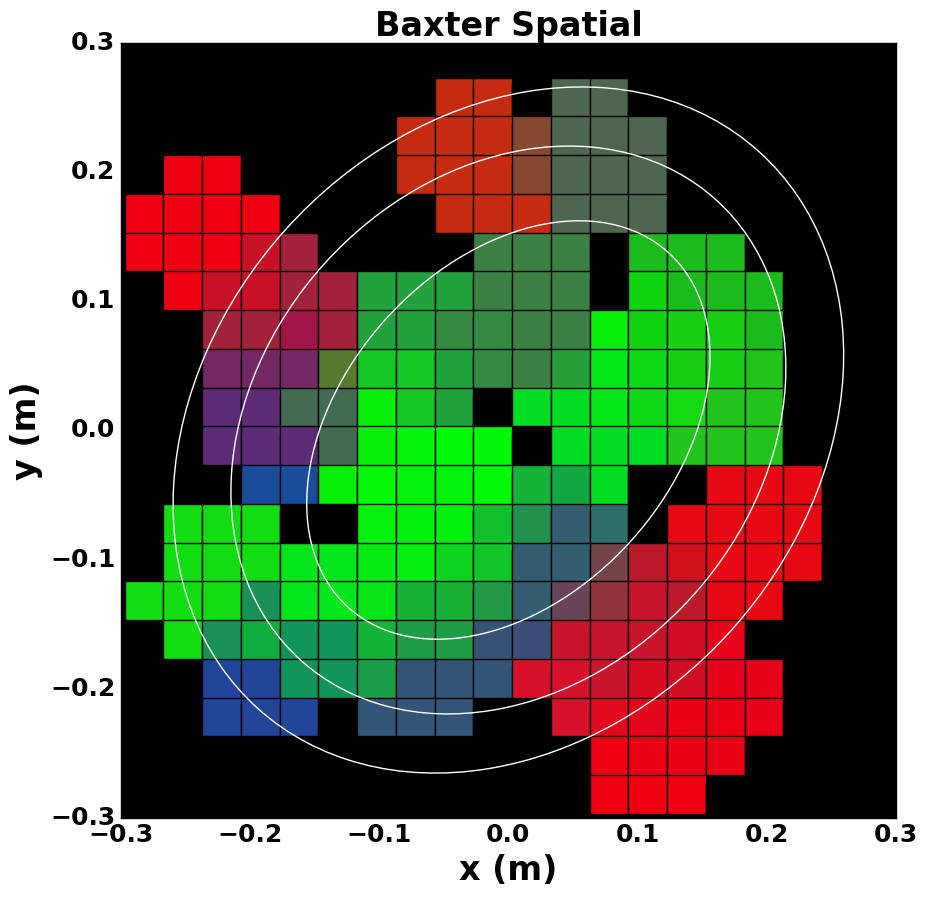
\includegraphics[width=0.4\textwidth ]{figures/baxter_Spatial__color.png}
%     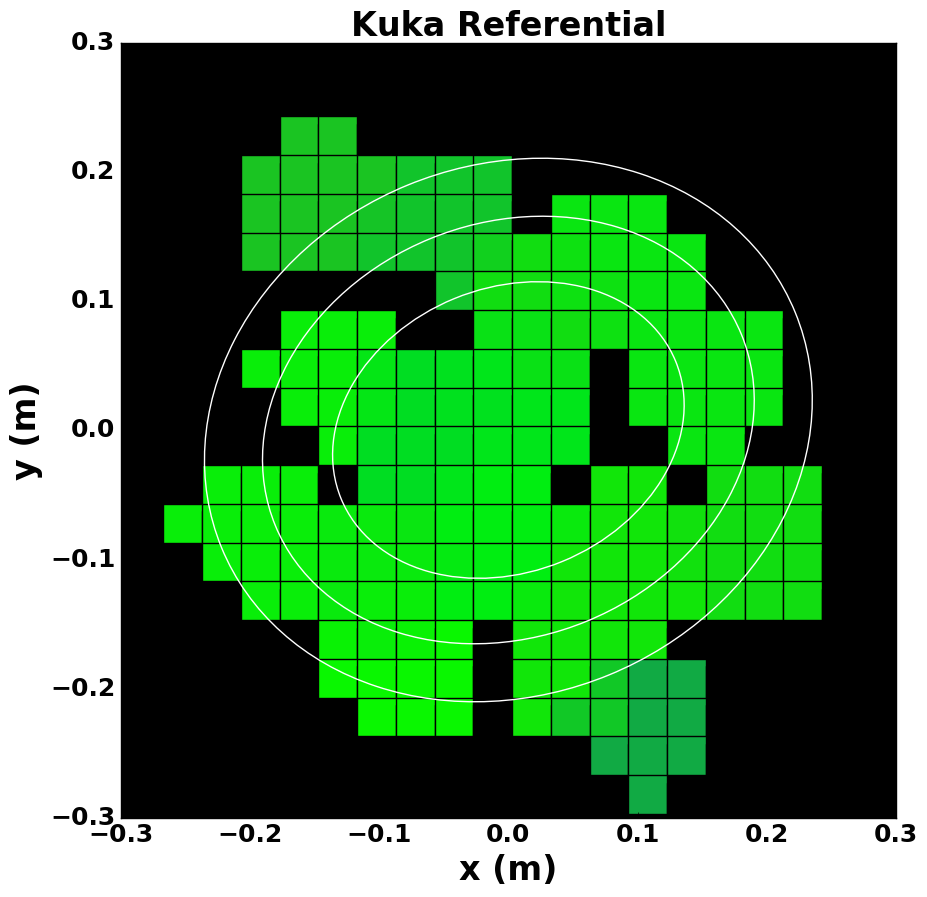
\includegraphics[width=0.4\textwidth ]{figures/kuka_Referential__color.png}
%     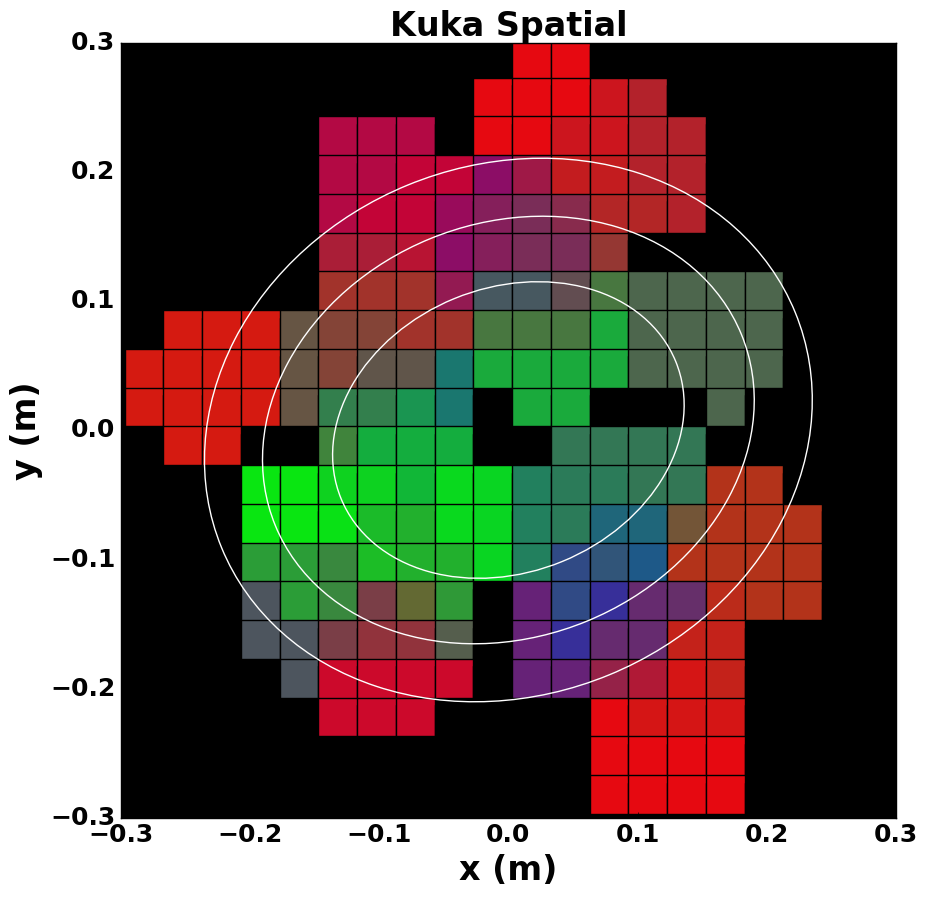
\includegraphics[width=0.4\textwidth ]{figures/kuka_Spatial__color.png}
%     \caption{The aggregated results from the referential versus spatial trials for the \textit{Baxter} and \textit{Kuka} robots. Each cell indicates the average responses over a $3\times3$ grid centered on it. The color represents the average fraction of correct responses as green, incorrect as red, and ambiguous ones as blue.}
%     \label{fig:colorsimple}
% \end{figure*}

\paragraph{Different verbs}  
To test if the effect is specific to the verb put, we designed a control experiment where everything remained the same as the Referential vs Spatial trials except the verb \textit{put} which we replaced with \textit{place, move} and \textit{push}. Here again 30 data points for each sampled $x^*$


\begin{figure*}[t!]
    \centering
    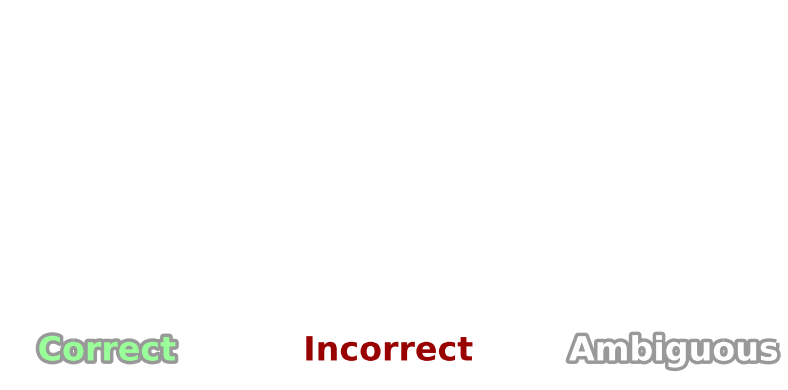
\includegraphics[width=0.5\textwidth, trim={0 0 0 3.3in},clip ] {figures/labels.png}\\
    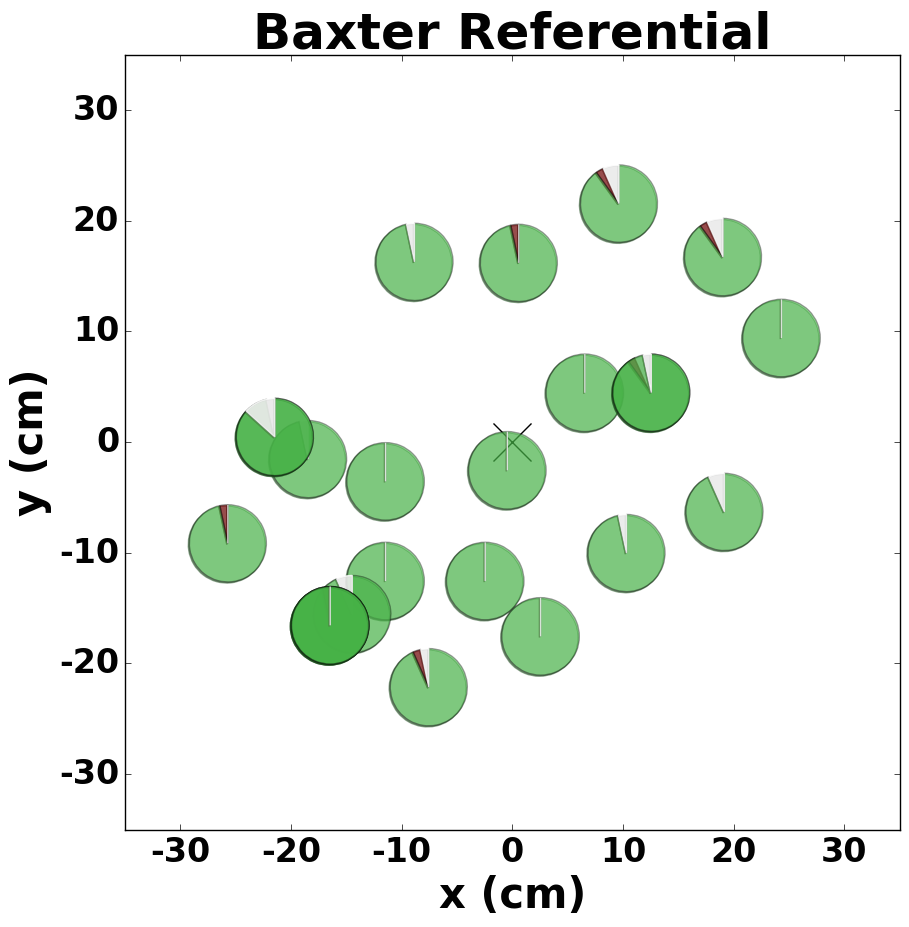
\includegraphics[width=0.32\textwidth ] {figures/baxter_Referential_.png}
    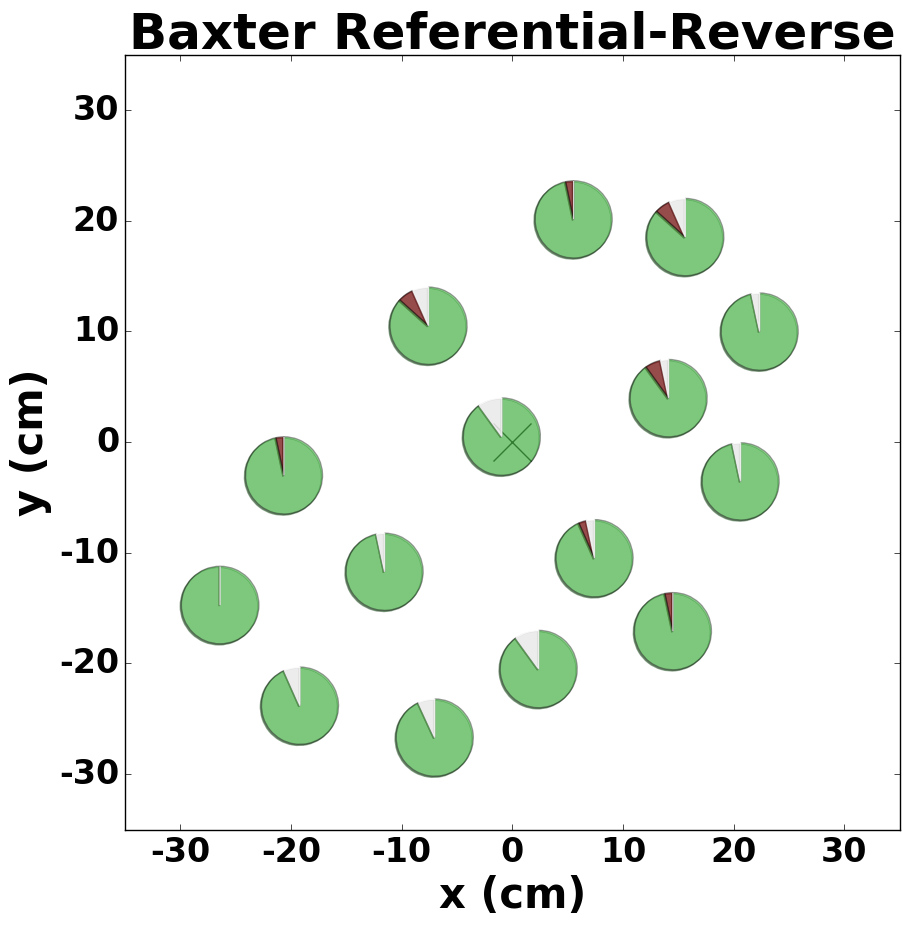
\includegraphics[width=0.32\textwidth ] {figures/baxter_Referential-Reverse_.png}
    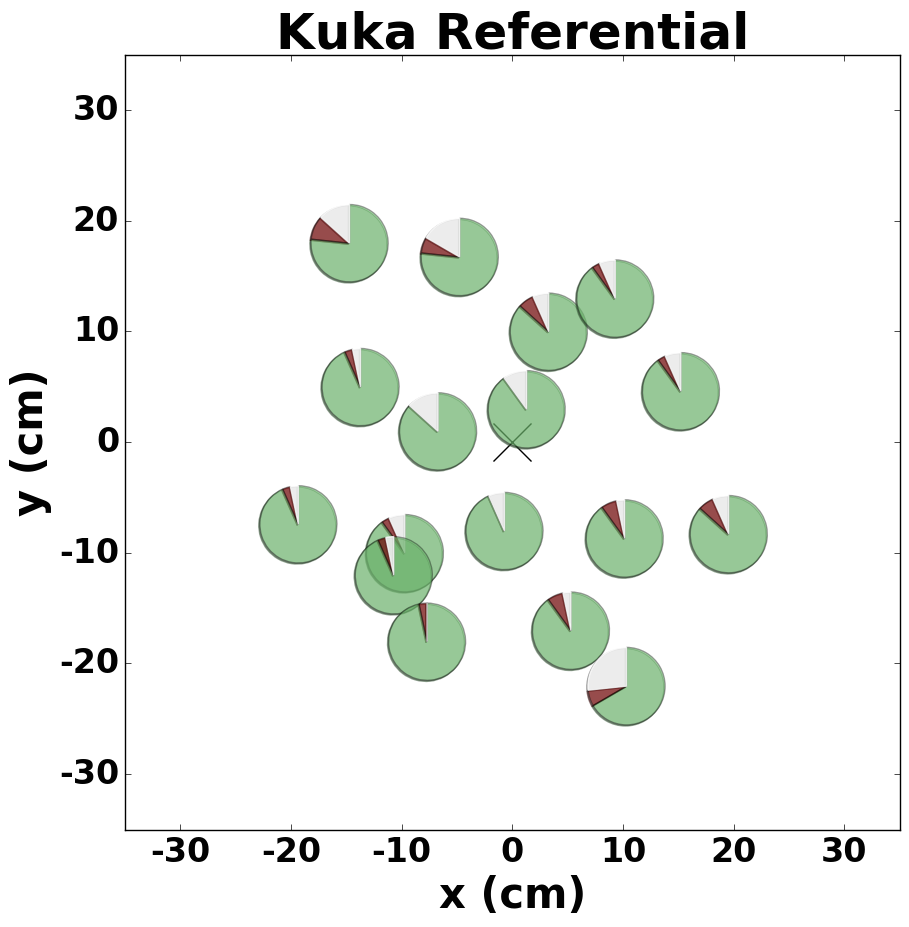
\includegraphics[width=0.32\textwidth ]{figures/kuka_Referential_.png}
    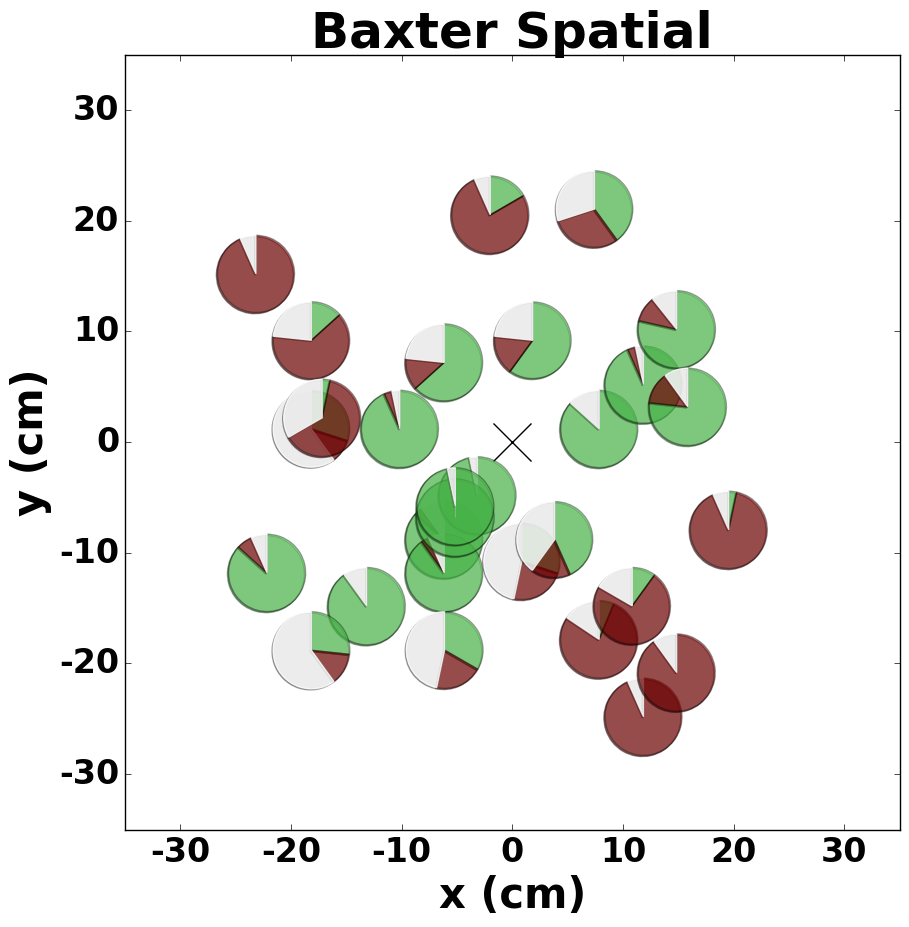
\includegraphics[width=0.32\textwidth ]{figures/baxter_Spatial_.png}
    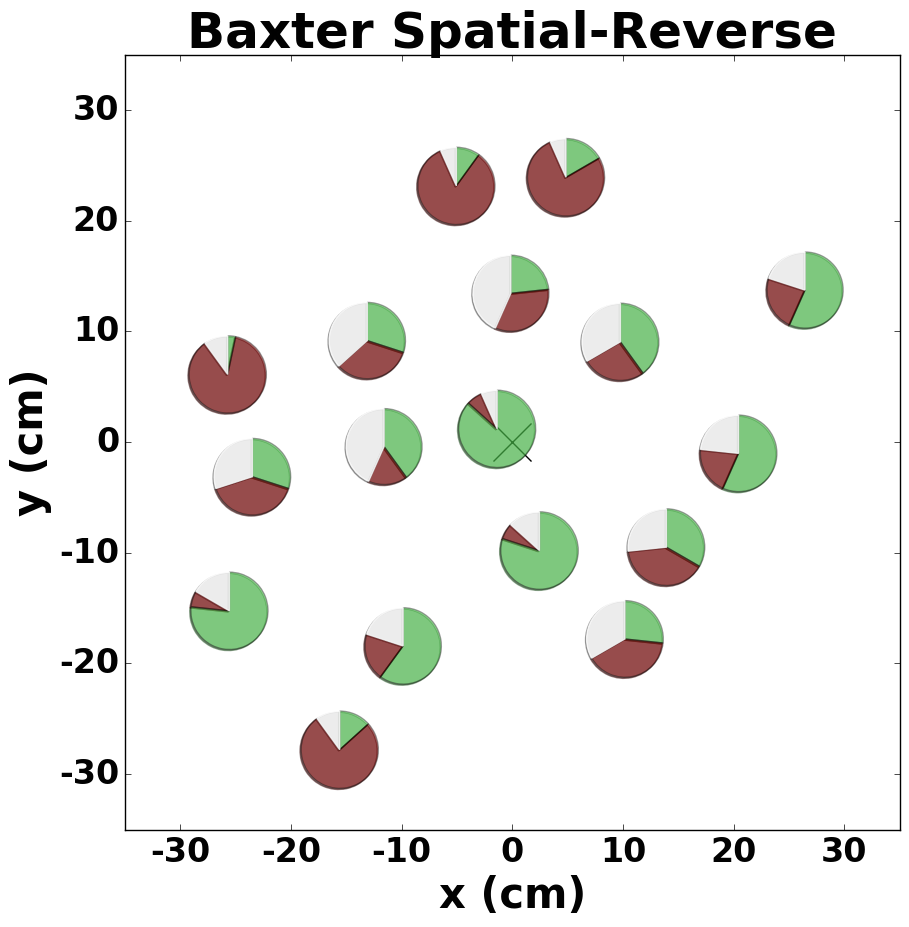
\includegraphics[width=0.32\textwidth ]{figures/baxter_Spatial-Reverse_.png}
    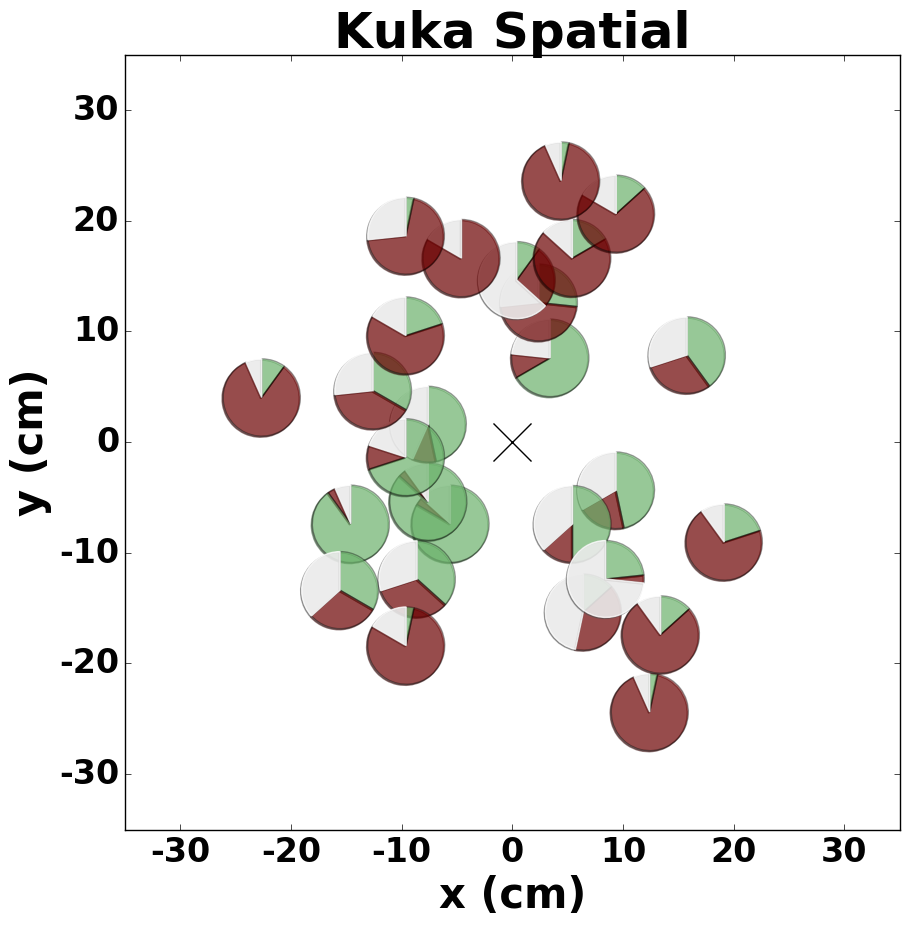
\includegraphics[width=0.32\textwidth ]{figures/kuka_Spatial_.png}
    \caption{The aggregated results from the referential versus spatial trials for the \textit{Baxter} and \textit{Kuka} robots. The locations of the responses correspond to the center of the circles, and are plotted in the coordinate frame centered at the position of the pointing action, marked with $\times$. The circles show the fraction of correct (grey), incorrect(black) and ambiguous(white) responses.}
    \label{fig:aggregatesimple}
\end{figure*}


% \begin{figure}[h]
%     \centering
%     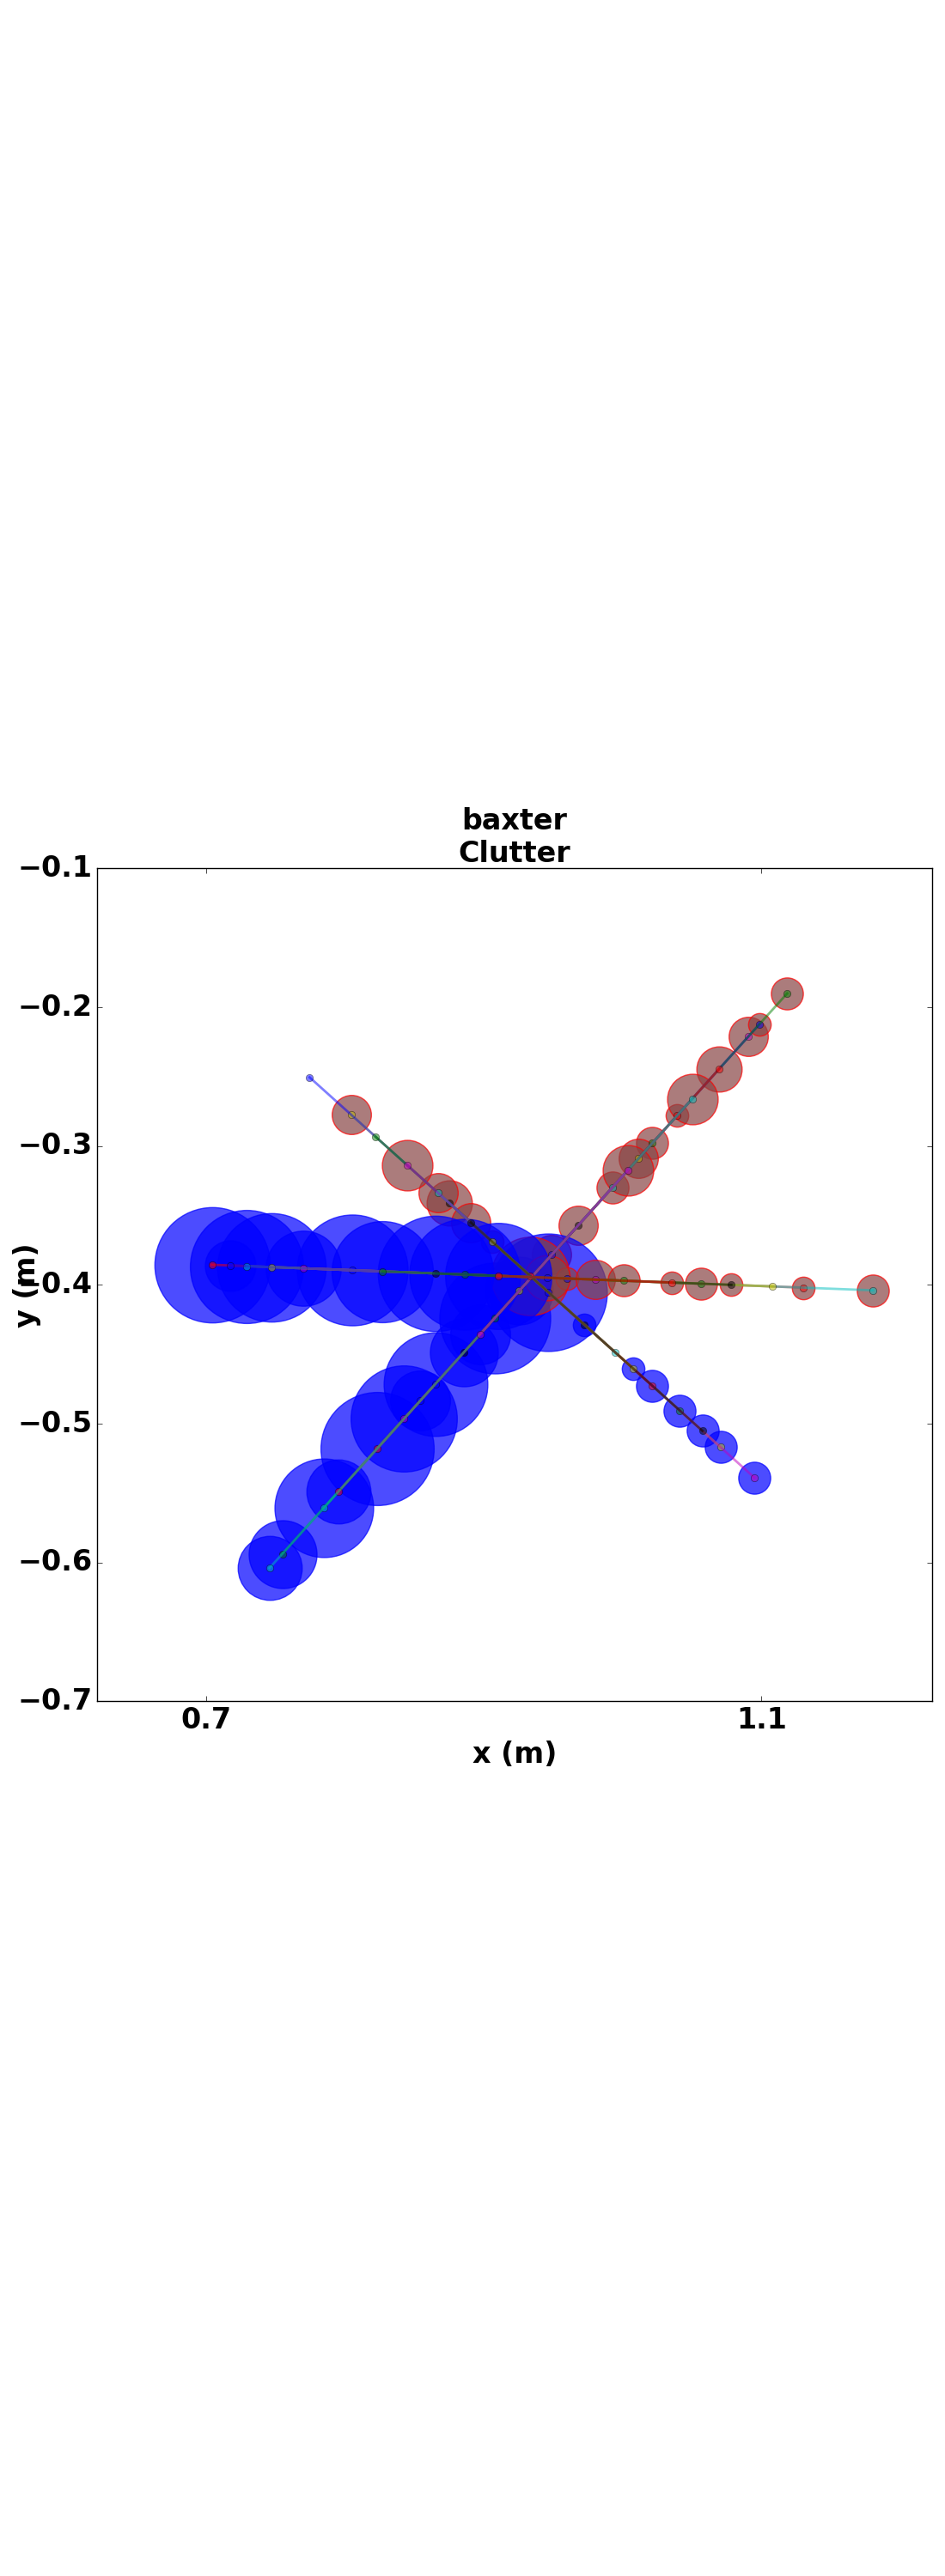
\includegraphics[width=0.47\textwidth ] {figures/baxter_Clutter_clutter.png}
%     \caption{The aggregated results from the cluttered scene trials for the \textit{Baxter} robot. The locations of the responses correspond to the center of the circles, and are plotted in the coordinate frame centered at the position of the true pointing action, marked with $\times$. Each circle shows the fraction of responses for cup 1 (red), and cup 2 (blue).}
%     \label{fig:baxterclutter}
% \end{figure}

\paragraph{Referential vs Spatial}
We study how varying the target of the pointing action from a referent object to a part of the space changes the interpretation of the pointing action by comparing the interpretation of the position of the pointing action $x^*$ in each condition. 
% $x^*$ represent the area on the table that contains the correct target of the pointing action. 


Figure~\ref{fig:aggregatesimple} shows the results of the experiment. The plot shows the spread of \textit{correct, incorrect, ambiguous} responses over the sampled positions about the location of a referential, and spatial pointing action. The referential data demonstrates the robustness of the interpretation. Most of the responses were overwhelmingly \textit{'correct'}, for both robots in interpreting a referent object in the \textit{pick} part of a pick-and-place task. The spatial pointing shows a much higher sensitivity to an accuracy of $x^*$ with respect to the true final placement. This comes up as a larger incidence of \textit{'incorrect'} and \textit{'ambiguous'} responses from the human subjects. This trend is true for the reverse trial as well.

While the study attempts to separate out and measure the critical aspects of the interpretation of robotic pointing actions some ambiguities like those arising out of perspective of the camera being projected onto a simulated 2D video or image are unavoidable. We suspect that the stretch of the 'correct' response green regions in the spatial plots is due to this perspective issue.

To test our hypothesis, we performed a Chi-squared test and compared the proportion of \textit{correct}, \textit{incorrect} and \textit{ambiguous} responses in referential and spatial trials. The results of the test shows that these two classes are statistically significantly different ($\chi^2= 13.89, p = 0.00096$).

To study if we are observing the same effects in the results of the reverse trial, no speech trial and the Kuka trial, we ran an equivalence test on the third hypothesis following the two one-sided tests method as described in \cite{lakens2017equivalence}, where each test is a pooled z-test with no continuity
correction with a significance level of 0.05. We found that changing the robot, removing the speech and the direction of the pointing action does not make a difference in the interpretation of spatial pointing and referential pointing within any margin that is less than 5\%.



\paragraph{Natural vs Unnatural}

We observed in the natural scene, when the end-effector points towards the edge of the cube that is on top of the stack, subjects place the new cube on top of the stack or on the table instead of the edge of the cube. However, in the unnatural scene, when we explain for subjects that there is no gravity, majority of them agree with the final image that has the cube placed on the edge of the cube. Table~\ref{tab:natural-unnatural} presents the results of this experiment. 

\begin{figure}[H]
% \vspace{-0.3in}
    \centering
    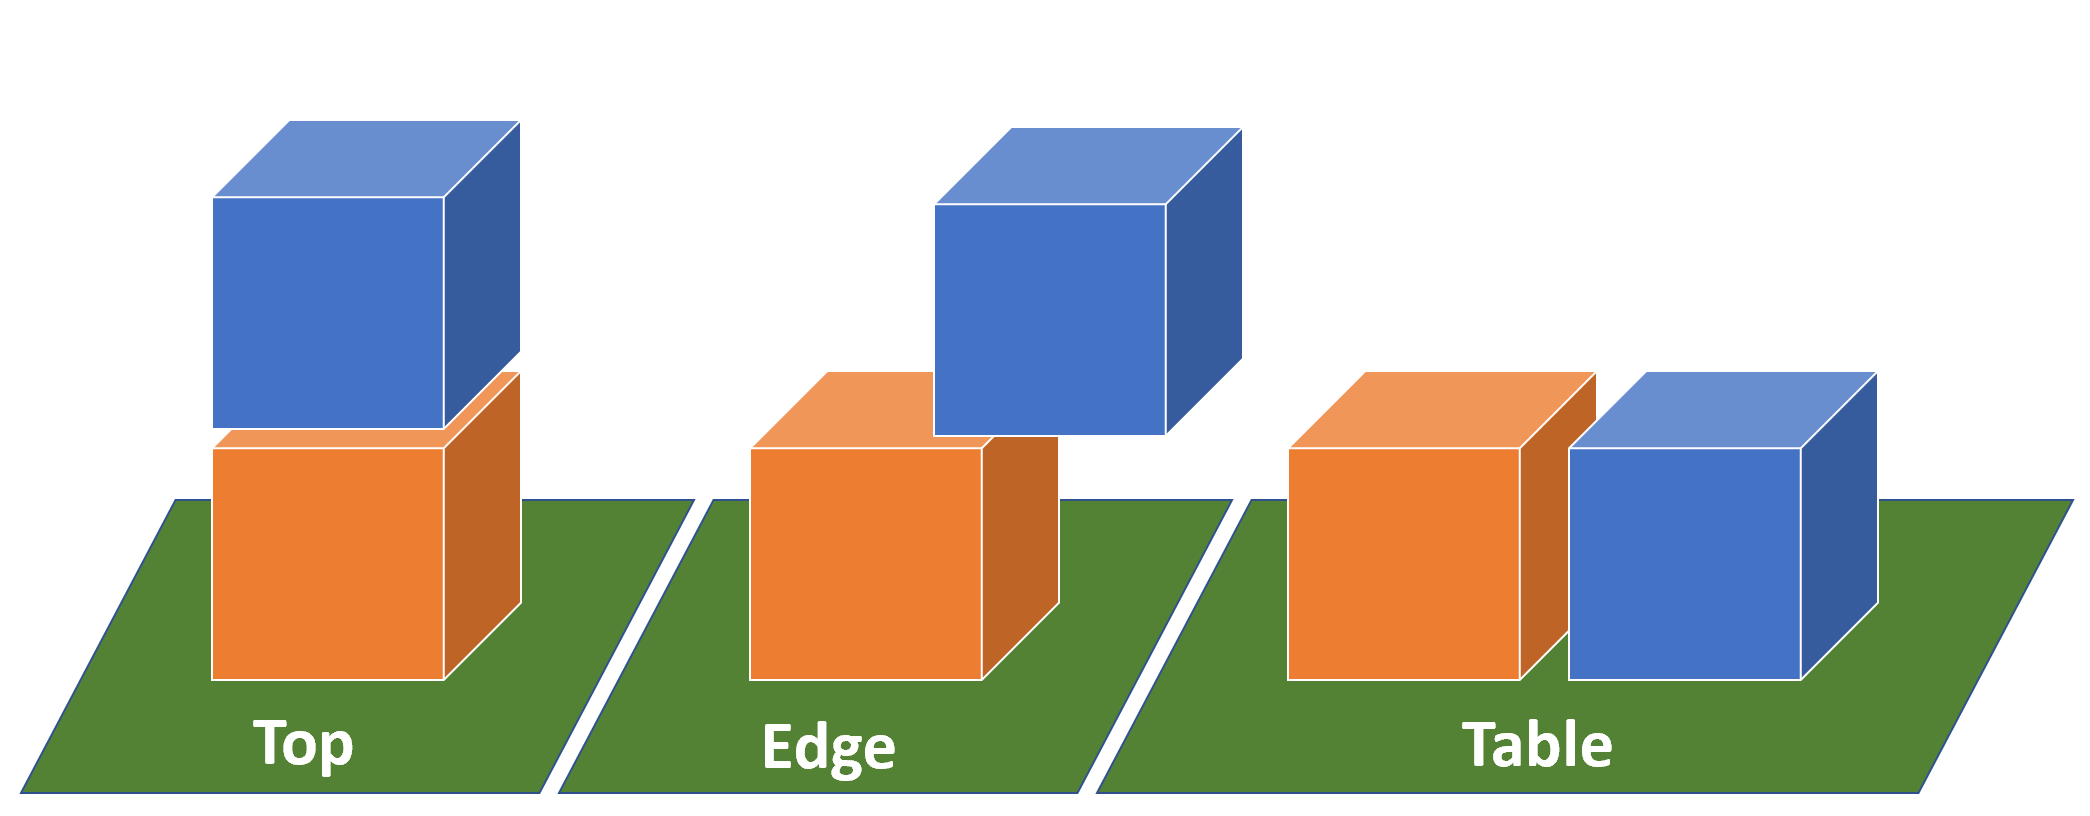
\includegraphics[width=0.4\textwidth, trim={0 0 0 0.7in},clip ] {figures/topedgetable.png}
    \vspace{-0.1in}
    \caption{
    The diagram shows the three different configurations of the placement of a blue cuboid object evaluated in the \textit{Natural vs Unnatural} trials. 
    % (\textit{Left:}) The object lies on top; (\textit{Middle:}) The object lies in an unstable manner off the edge;  (\textit{Right:}) The object lies beside on the table.
    }
    \label{fig:topedgetable}
    \vspace{-0.2in}
\end{figure}


\begin{table}[H]
\centering
\begin{tabular}{lllll}
& \multicolumn{1}{l}{} & \multicolumn{1}{l}{correct} & \multicolumn{1}{l}{incorrect} & ambiguous \\ \hline
\multicolumn{1}{l}{\multirow{unnatural}} & top                   & 12                           & 9                              & 9         \\
\multicolumn{1}{l}{}                           & \textbf{edge}                  & \textbf{24}                           & 2                              & 4         \\
\multicolumn{1}{l}{}                           & table                 & 2                            & 2                              & 26        \\ \hline
\multicolumn{1}{l}{\multirow{natural}}   & \textbf{top }                  & \textbf{26}                           & 3                              & 1         \\
\multicolumn{1}{l}{}                           & edge                  & 9                            & 11                             & 10        \\
\multicolumn{1}{l}{}                           & table                 & 7                            & 13                             & 12        \\ \hline
\end{tabular}
\caption{Results of the unnatural scene and natural scene. (numbers are our of 30) }
\label{tab:natural-unnatural}
\end{table}


\begin{figure}[H]
    \centering
    % 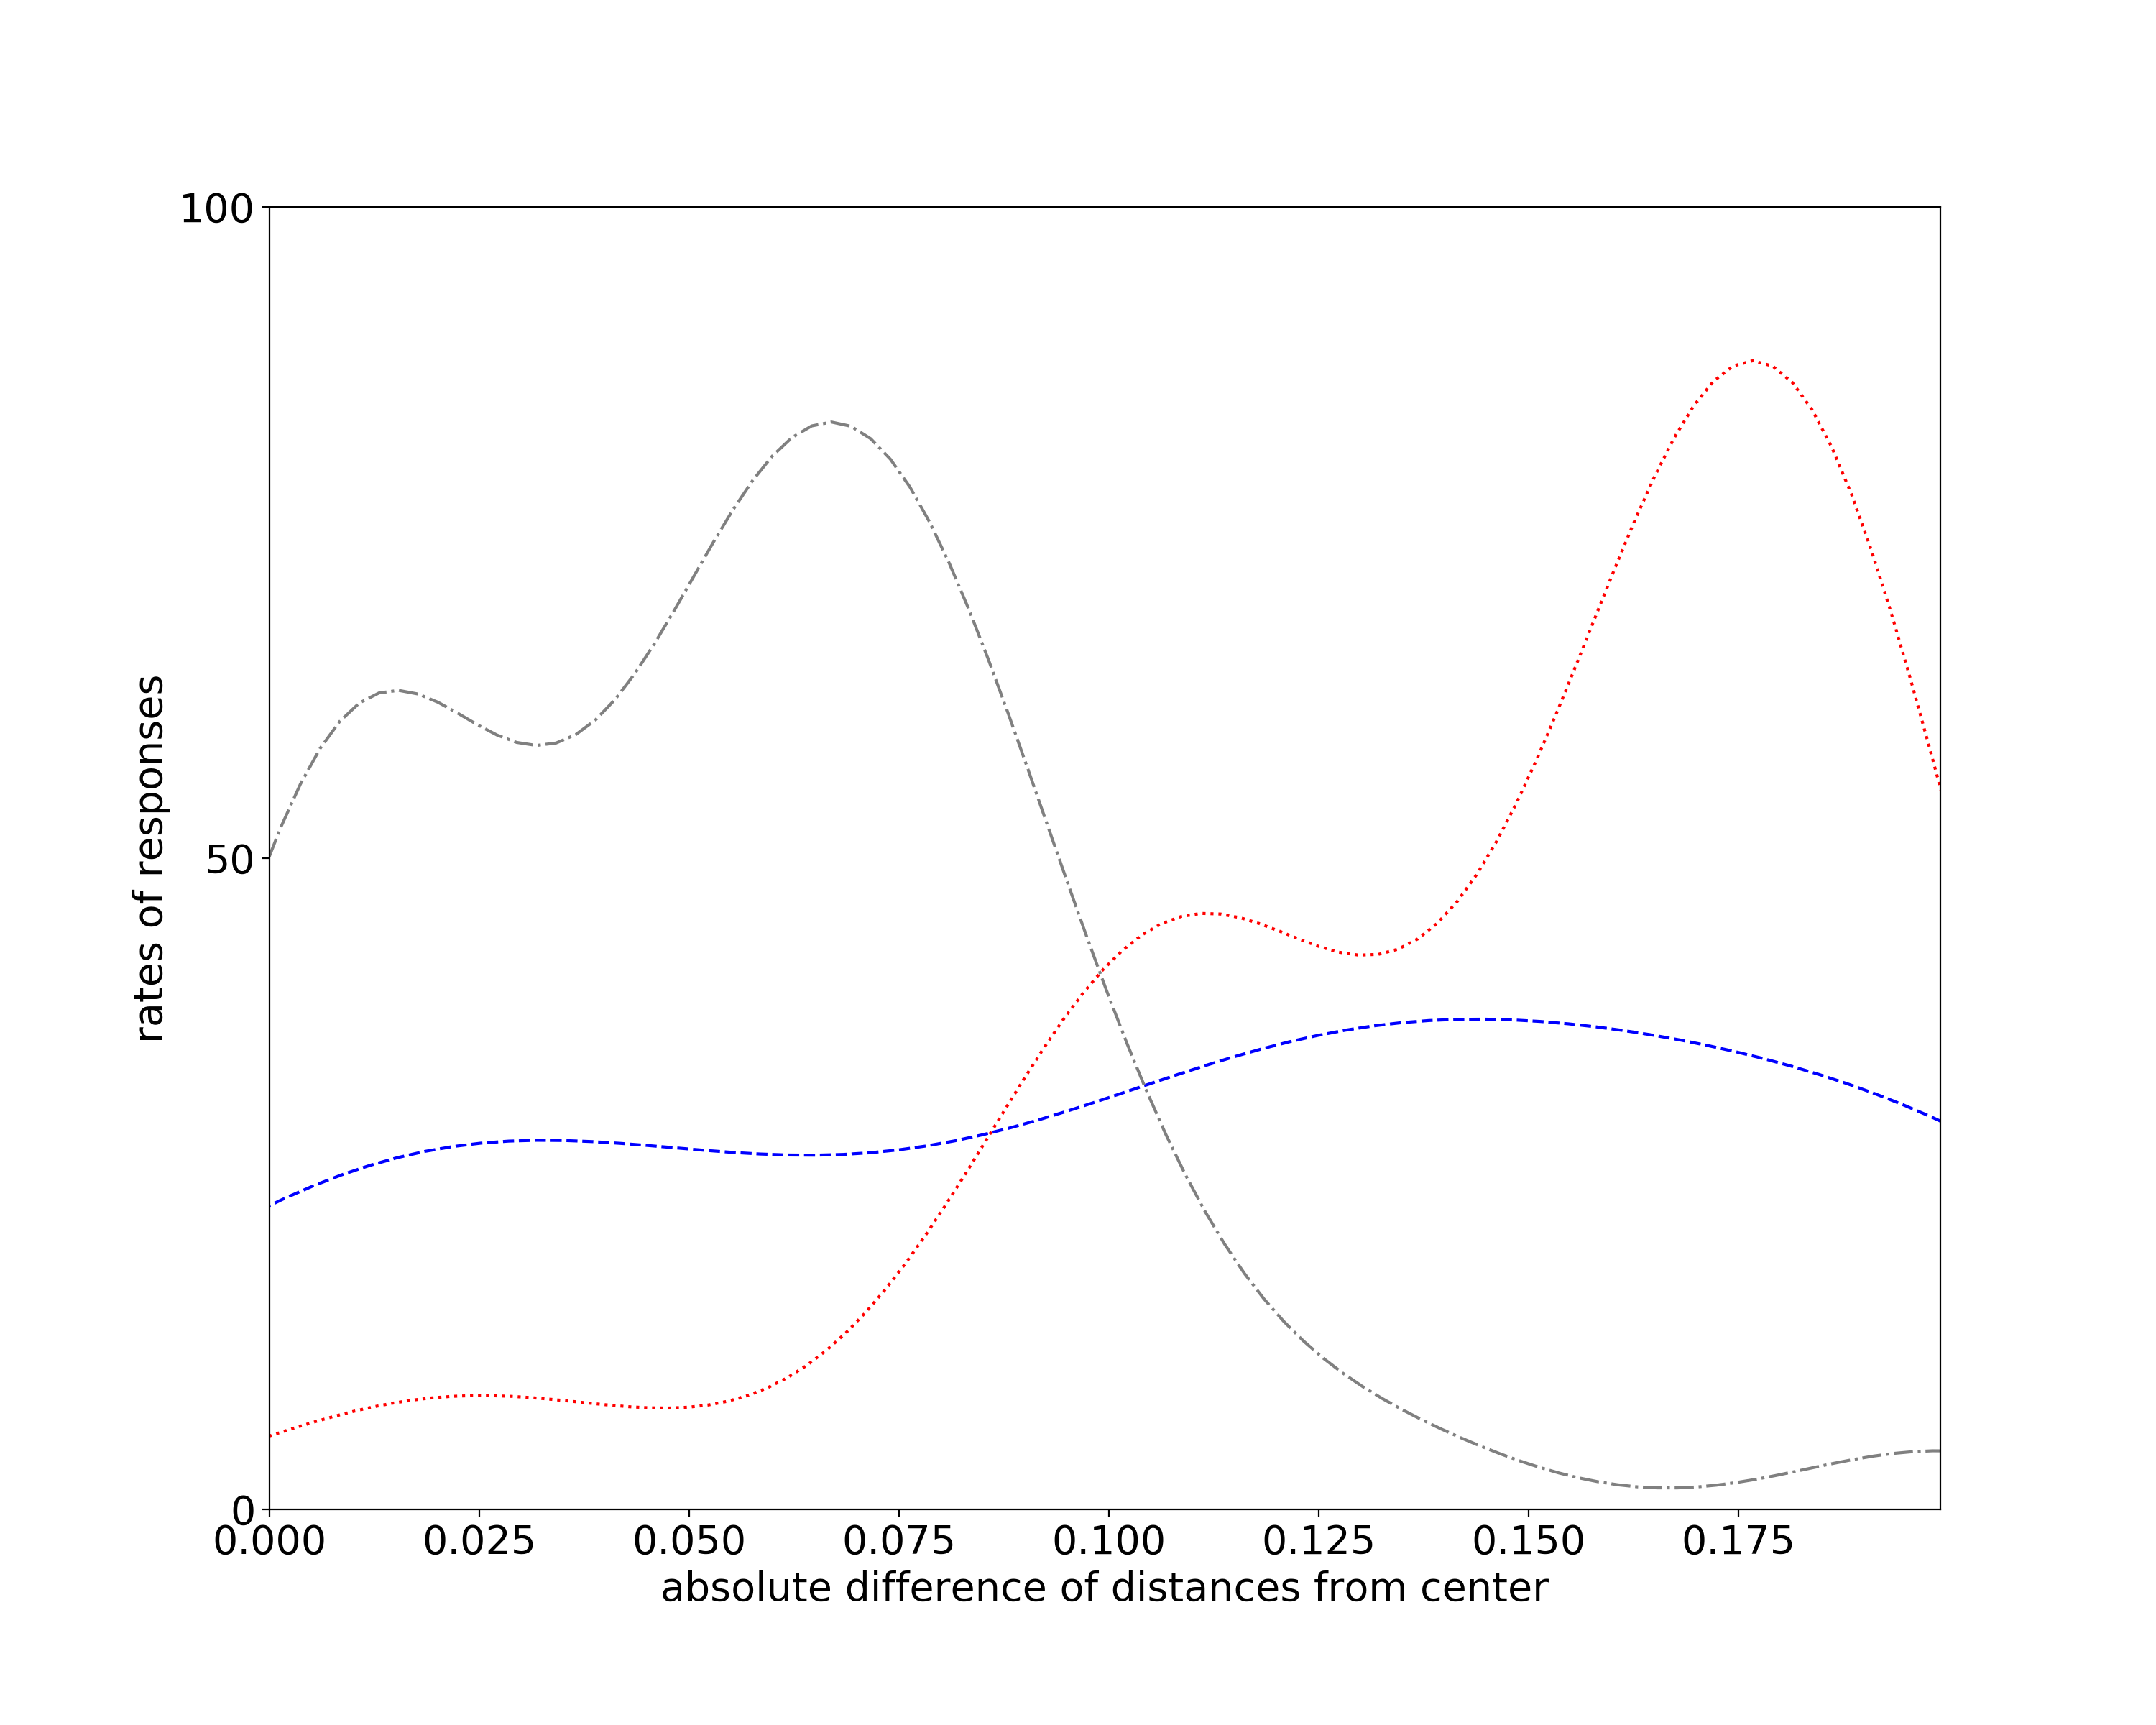
\includegraphics[height=0.23\textwidth]{cluttered-malihe.png}
    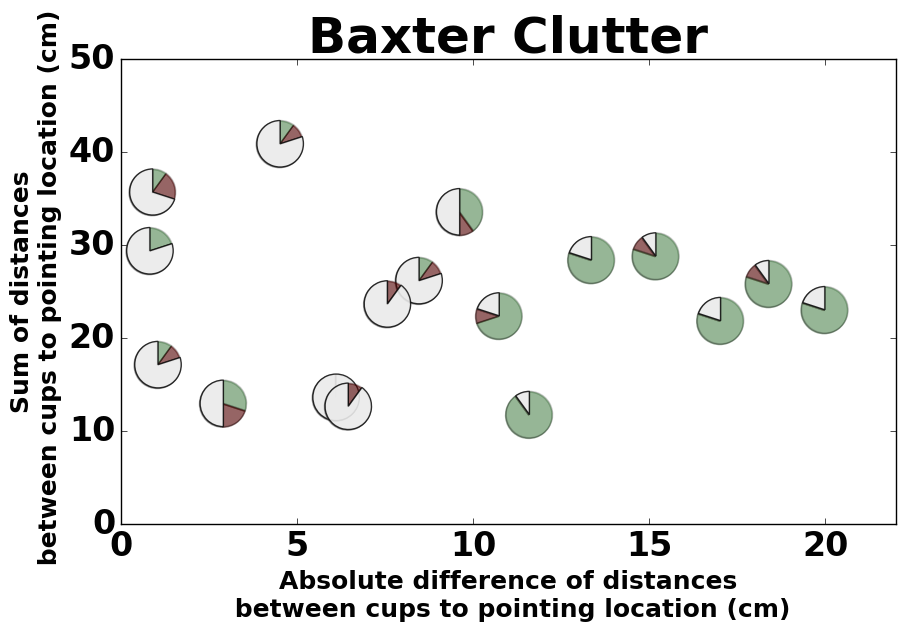
\includegraphics[width=\linewidth]{figures/baxter_Clutter_granular.png}
    % 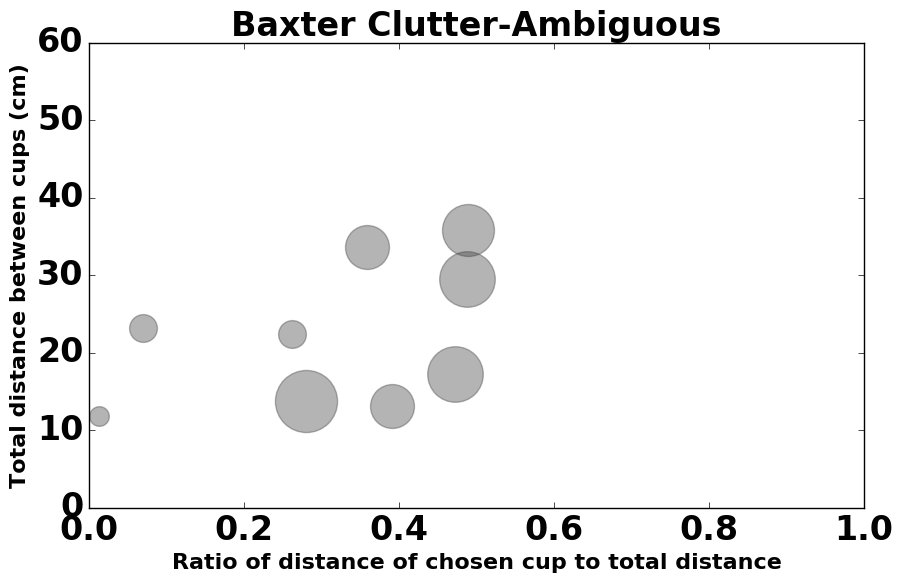
\includegraphics[width=0.35\textwidth]{figures/baxter_Clutter-Ambiguous2_granular.png}
    \caption{
    % (\textit{Top:} Histogram of responses in the cluttered scene. Red represents responses that correspond to the nearer object. Blue represents the farther object. Gray shows ambiguous responses. (\textit{Bottom:}) )
    The scatter plot represents the spread of responses where human subjects chose the \textit{nearer cup} (green), \textit{farther} cup (red), and ambiguous (grey). 
    The \textit{x-axis} represents the absolute difference between the distances of each cup to the locations of pointing, the \textit{y-axis} represents the total distance between the two cups.
    }
    \label{fig:cluttered}
\end{figure}

\paragraph{Different verbs}
The results of the Chi-squared test shows that in Spatial trials when we replace \textit{put} with \textit{place}, \textit{push} and \textit{move}, the differences of the distributions of \textit{correct}, \textit{incorrect} and \textit{ambiguous} responses are not statistically significant ($\chi=0.2344 $, $p = 0.971$). The coefficients of the multinomial logistic regression model and the p-values suggest that the differences in judgements for each sampled point with different verbs are not statically significant ($b<0.0001$ , $p>0.98$).



\paragraph{Cluttered}

% \begin{figure}[t!] what are those two blocks, give it we are going to attempt to come up with a principles that explain our observation
%     \centering
%     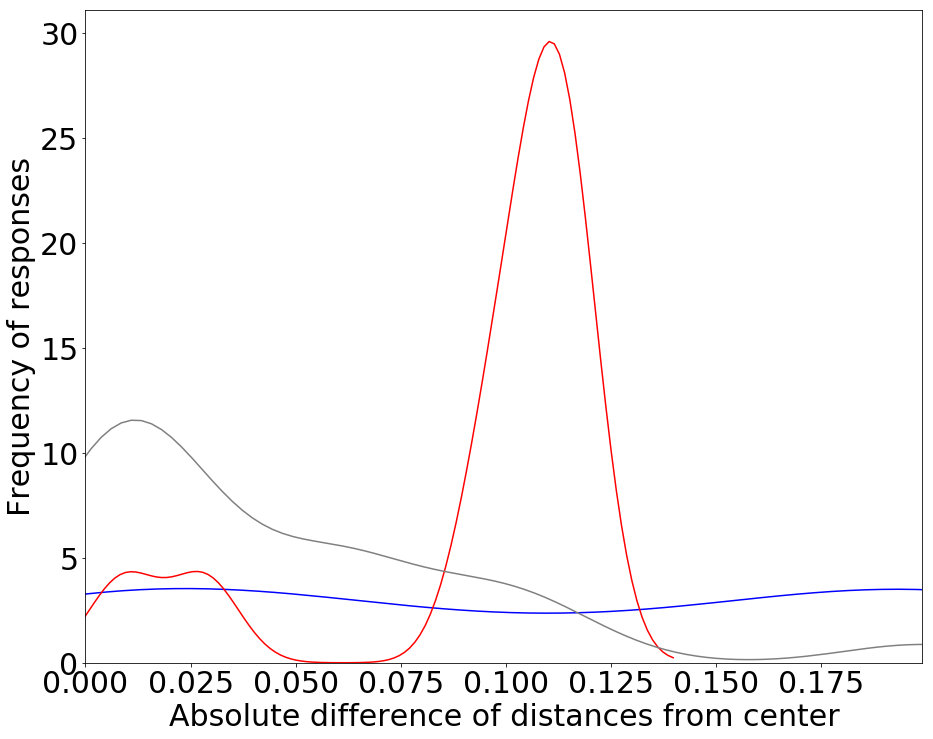
\includegraphics[width=0.3\textwidth]{figures/cluttered-histogram.png}
%     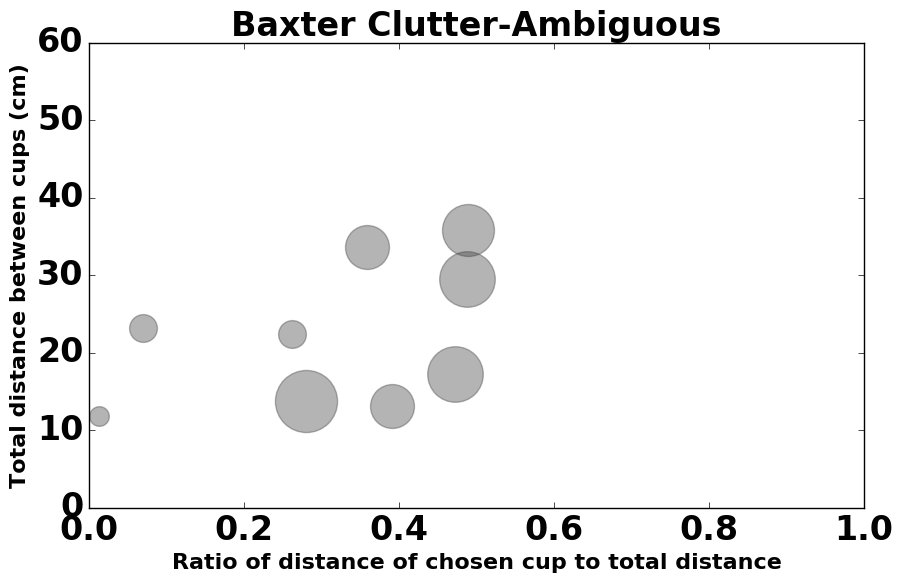
\includegraphics[width=0.35\textwidth]{figures/baxter_Clutter-Ambiguous2_granular.png}
%     \caption{(\textit{Top:} Histogram of responses in the cluttered scene. Red represents responses that correspond to the nearer object. Blue represents the farther object. Gray shows ambiguous responses. (\textit{Bottom:}) The scatter plot shows the ratio of the distance of a nearer object in an ambiguous response to the total distance, plotted against the total distance between objects. Most of these happen when the objects are too close to (close to the X axis), or equidistant from the pointing location (around the ratio of 0.5).)}
%     \label{fig:cluttered}
% \end{figure}



As we can see in Figure~\ref{fig:cluttered}, the higher is the absolute difference of centers of distances from the center, the more likely it is that subjects pick a mug (green or red) as opposed to the \textit{ambiguous} choice. That is when the two mugs were very close, almost next to each other (less than 10 cm apart), majority of subjects chose the \textit{ambiguous} option. 
 
% The blue line in Figure~\ref{fig:cluttered} shows the frequency of the cases 
% The red sections of the circles indicates responses
% when 

When the target is not very close to the distractor, and when the pointing finger points towards $x^*$ on the table that is closer to one mug, subjects picked the mug that was the correct target of the pointing action more often than the incorrect one. This was true for all of the cases in our dataset. Referential pointing is flexible. Even in the presence of a distractor, there is not need for accurate exact pointing, as long as the target object is not ambiguous, people interpret the pointing action correctly.






% \paragraph{speech}
% We study how varying the target of the pointing action from part of the space to a target object changes the interpretation of the pointing action by comparing the value of x* in each condition. $x^*$ represent the area on the table that contains the correct target of the pointing action. 



% To test our hypothesis, we will perform proportion test (two-tailed z-test) and the t-test in the exploratory analysis in case it is needed. 
% Another way to test this idea is through a logistic regression where the dependent variable is a binary variable indicating whether or not the pointing action is understood correctly, and the independent variable is $x^*$. In this regression framework, our hypothesis states that the coefficient of $x^*$ would be insignificant. 
% To study the values that $x^*$ can take, we randomly select 8 points in each quadrant in the circle that is the intersection of the cone that comes out of the index finger and the surface of the table.

  


% \begin{figure}
%     \centering
%     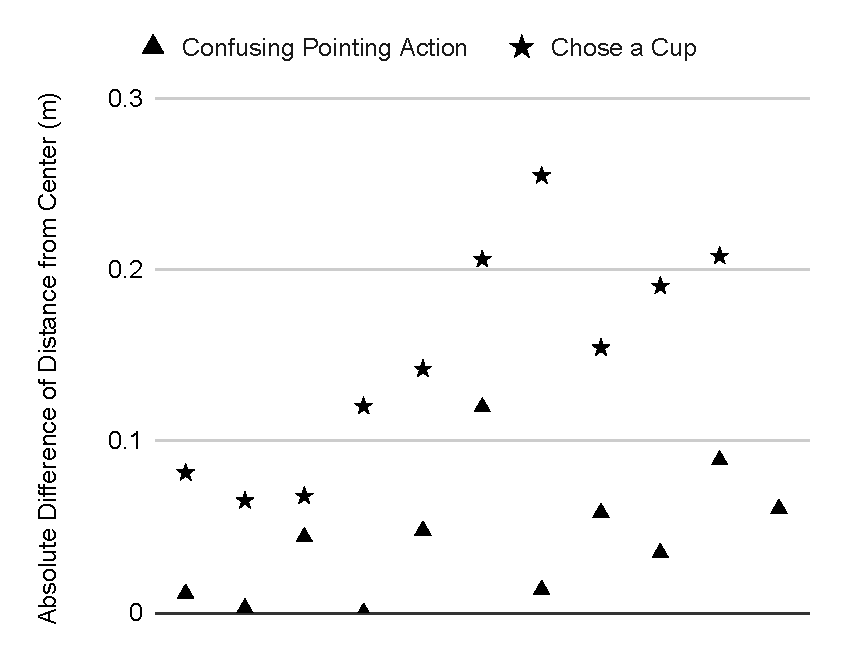
\includegraphics[width= \linewidth]{line_difference_chart (1).pdf}
%     \caption{Cluttered scene results}
%     \label{fig:line_figure}
% \end{figure}


% \begin{figure}
%     \centering
%     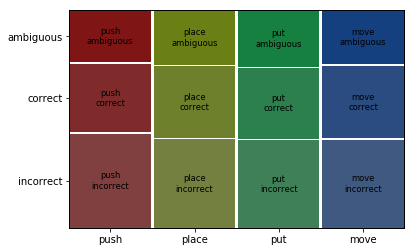
\includegraphics[width=\linewidth]{verbs.png}
%     \caption{different verbs}
%     \label{fig:verbs}
% \end{figure}



%  For instance in Figure~\ref{fig:aggregatesimple}, the 'correct' spatial responses are \textit{stretched} because of perspective. 
 
%  $ \epsilon = (\epsilon_1, \epsilon_2)$.
 


% \paragraph{Case 3: Referring expressions with pointing}

% $(x^*,RE), RE \subseteq \{ o_1, \dots, o_N \}  $ then \\
% Intended Object $= \argmin_{O \in RE} |O-x^*|$


% \paragraph{Case 3: Commonsense, Natural vs Unnatural}
% CS: constraints on possible interpretations of pointing action\\
% IR: Interpretation of pointing action= action of the addressee \\

% $IR \in CS$






\section{Human Evaluation of Instructions}

After designing and conducting our experiments, we became concerned that subjects might regard imprecise referential pointing as understandable but unnatural.  If they did, their judgments might combine ordinary interpretive reasoning with additional effort, self-consciousness or repair.  We therefore added a separate evaluation to assess how natural the generated pointing actions and instructions are. We recruited 480 subjects from Mechanical Turk using the same protocol described in our Data Collection procedure, and asked them to rank how natural they regarded the instruction on a scale of \textit{0 to 5}. 

The examples were randomly sampled from the videos of the referential pointing trials that we showed to subjects for both the Baxter and Kuka robots. These examples were selected in a way that we obtained equal number of samples from each cone. The average rating for samples from the $\ang{45}$, $\ang{67.5}$ and $\ang{90}$ cone are $3.625, 3.521$
and $3.650$ respectively. For Kuka, the average rating for samples from the $\ang{45}$, $\ang{67.5}$ and $\ang{90}$ cone are $3.450, 3.375$, and $3.400$. Overall, the average for Baxter is $3.600$, and for Kuka is $3.408$. The differences between Kuka and Baxter and the differences across cones are not statistically significant ($t \leq |1.07|, p > 0.1 $).  Thus we have no evidence that subjects regard imprecise pointing as problematic.
% Malihe: exact numbers are:
% $t \leq |1.07|, p \geq 0.88 $
\\
\section{Design Principles}

The results of the experiments suggest that spatial pointing is interpreted rather precisely, where referential pointing is interpreted relatively flexibly.  This naturally aligns with the possibility for alternative interpretations.  For spatial reference, any location is a potential target.  However, for referential pointing, it suffices to distinguish the target object from its distractors.

We can characterize this interpretive process in formal terms by drawing on observations from the literature on vagueness \cite{kyburg2000fitting,graff2000shifting}.  Any pointing gesture starts from a set of candidate interpretations $D \subset \mathcal{W}$ determined by the context and the communicative goal.  In unconstrained situations, spatial pointing allows a full set of candidates $D = \mathcal{W}.$  If factors like common-sense physics impose task constraints, that translates to restrictions on feasible targets $CS$, leading to a more restricted set of candidates $D = CS \cap \mathcal{W}$.  Finally, for referential pointing, the potential targets are located at locations $x_1 \ldots x_N \in S$, and $D = \{ x_1 \ldots x_N \}.$

Based on the communicative setting, we know that the pointing gesture, like any vague referring expression, must select at least one of the possible interpretations \cite{kyburg2000fitting}.  We can find the best interpretation by its distance to the target $x^*$ of the pointing gesture.  Using $d(x,x^*)$ to denote this distance, gives us a threshold $$\theta = \min_{x \in D} d(x, x^*).$$

Vague descriptions can't be sensitive to fine distinctions \cite{graff2000shifting}.  So if a referent at $\theta$ is close enough to the pointing target, then another at $\theta + \epsilon$ must be close enough as well, for any value of $\epsilon$ that is not significant in the conversational context.  Our results suggest that viewers regard 10cm (in the scale of the model simulation) as an approximate threshold for a significant difference in our experiments.

In all, we predict that a pointing gesture is interpreted as referring to $\{x \in D | d(x,x^*) \leq \theta + \epsilon\}.$  We explain the different interpretations through the different choice of $D$.

\paragraph{Spatial Pointing.}  For unconstrained spatial pointing, $x^* \in D$, so $\theta=0$.  That means, the intended placement cannot differ significantly from the pointing target.  Taking into account common sense, we allow for small divergences that connect the pointing, for example, to the closest stable placement.

\paragraph{Referential Pointing.}  For referential pointing, candidates play a much stronger role.  A pointing gesture always has the closest object to the pointing target as a possible referent.  However, ambiguities arise when the geometries of more than one object intersect with the $\theta+\epsilon$-neighborhood of $x^*$.   We can think of that, intuitively, in terms of the effects of $\theta$ and $\epsilon$.  Alternative referents give rise to ambiguity not only when they are too close to the target location ($\theta$) but even when they are simply not significantly further away from the target location ($\epsilon$).  

\section{Conclusion}
\label{conclusion}

We have presented an empirical study of the interpretation of simulated robots instructing pick-and-place tasks.  Our results show that robots can effectively combine pointing gestures and spoken instructions to communicate both object information and spatial information---and offer the first empirical characterization of the use of robot gestures to communicate precise spatial locations.  The dataset and a demo of the experiments are attached with this submission, and will be released upon acceptance of the paper.  We have suggested that pointing, in line with other vague references, select from a set of candidate interpretations that depend on the task, context and communicative goal.  They pick those candidates that are not significantly further from the pointing ray than the best ones.  This contrasts with previous models that required pointing gestures to target a referent exactly or fall within a context-independent pointing cone.

Our work has a number of limitations that suggest avenues for future work.   It remains to implement our design principles on robot hardware, explore the motion planning problems associated with generating imprecise but interpretable gestures, and verify the interpretations of physically copresent viewers.  Note that we used a 2d interface, which can introduce artifacts, for example from the effect of perspective.  In addition, robots can in general trade off pointing gestures with other descriptive material in offering instructions.  Future work is needed to assess how such trade-offs play out in spatial reference, not just in object reference.


\bibliography{pointing.bib} 
\bibliographystyle{aaai}
\end{document}